% changelog: "1.2.0, 2024-08-10, Stesura UC-0, UC-1 e UC-5.12. Aggiunta requisiti, Veronica Tecchiati"
\documentclass[8pt]{article}
\usepackage[italian]{babel}
\usepackage[utf8]{inputenc}
\usepackage[letterpaper, left=1in, right=1in, bottom=0.75in, top=0.75in]{geometry}
\usepackage[table]{xcolor}
\usepackage{amsmath}
\usepackage{subfiles}
\usepackage{lipsum}
\usepackage{csquotes}
\usepackage{amsfonts}
\usepackage[sfdefault]{plex-sans}
\usepackage{float}
\usepackage{pifont}
\usepackage{mathabx}
\usepackage[euler]{textgreek}
\usepackage{makecell}
\usepackage{tikz, ifthen, xstring, calc, pgfkeys, pgfopts, tikz-uml}
\usepackage{wrapfig}
\usepackage{siunitx}
\usepackage{amssymb} 
\usepackage{tabularx}
\usepackage{longtable}
\usepackage{adjustbox}
\usepackage[document]{ragged2e}
\usepackage{floatflt}
\usepackage[colorlinks=true,linkcolor=nan1fyblue,urlcolor=nan1fyblue]{hyperref}
\usepackage{graphicx}
\setcounter{tocdepth}{4}
\usepackage{caption}
\usepackage{multicol}
\usepackage{tikz}
\setlength\parindent{0pt}
\captionsetup{font=footnotesize}
\usepackage{fancyhdr} 
\usepackage{graphicx}
\usepackage{capt-of}
\usepackage{booktabs}
\usepackage{varwidth}
\usepackage{verbatim}
\usepackage{array}

\newcolumntype{P}[1]{>{\centering\arraybackslash}p{#1}}

\definecolor{nan1fyblue}{RGB}{23,103,162}
\tikzumlset{fill usecase=white}

% -- TITOLO INTESTAZIONE -- %
\newcommand{\customtitle}{ANALISI DEI REQUISITI} % o ESTERNO

% -- STILE INTESTAZIONE -- %
\fancypagestyle{mystyle}{
	\fancyhf{} 
	\fancyhead[R]{
\includegraphics[height=1cm]{../../template/images/logos/NaN1fy_logo.png}} 
	\fancyhead[L]{\leftmark} 
	\renewcommand{\headrulewidth}{1pt} 
	\fancyhead[L]{\customtitle} 
	\renewcommand{\headsep}{1.3cm} 
	\fancyfoot[C]{\thepage} 
}

% -- PER LA FIRMA -- %
\newcommand{\signatureline}[1]{%
	 \par\vspace{0.5cm}
	\noindent\makebox[\linewidth][r]{\rule{0.2\textwidth}{0.5pt}\hspace{3cm}\makebox[0pt][r]{\vspace{3pt}\footnotesize #1}}%
}

% -- PER IL GLOSSARIO -- %
\newcommand{\glossterm}[1]{#1\textsuperscript{G}} % inserisci \glossterm{termine}

\begin{document}
\definecolor{myblue}{RGB}{23,103,162}
\begin{titlepage}
	\begin{tikzpicture}[remember picture, overlay]
		\node[anchor=south east, opacity=0.2, yshift = -4cm, xshift= 2em] at (current page.south east)
      {
\includegraphics[width=0.7\textwidth, trim=0cm 0cm 5cm 0cm, clip]{../../template/images/logos/Universita_Padova_transparent.png}}; 
		\node[anchor=north west, opacity=1, yshift = 4.2cm, xshift= 1.4cm, scale=1.6] at (current
      page.south west) {
\includegraphics[width=4cm]{../../template/images/logos/NaN1fy_logo.png}};
	\end{tikzpicture}
	
	\begin{minipage}[t]{0.47\textwidth}
		{\large{\textsc{Destinatari}}
			\vspace{3mm}
			\\ \large{\textsc{Prof. Tullio Vardanega}}
			\\ \large{\textsc{Prof. Riccardo Cardin}}
		}
	\end{minipage}
	\hfill
	\begin{minipage}[t]{0.47\textwidth}\raggedleft
		{\large{\textsc{Redattori}}
			\vspace{3mm}
			{\\\large{\textsc{Guglielmo Barison}\\}}
			{\large{\textsc{Davide Donanzan\\}}}
   {\large{\textsc{Oscar Konieczny}\\}}
			{\large{\textsc{Veronica Tecchiati}}}
			
		}
		\vspace{8mm}
		
		{\large{\textsc{Verificatori}}
			\vspace{3mm}
			{\\\large{\textsc{Linda Barbiero}\\}}
                {\large{\textsc{Pietro Busato}\\}}
                {\large{\textsc{Oscar Konieczny}\\}} 
                {\large{\textsc{Davide Donanzan}\\}}
                {\large{\textsc{Veronica Tecchiati}\\}}
                {} %PER RIMUOVERE LO SPAZIO INDESIDERATO ALLA FINE DELL'ULTIMO NOME, ANDARE A CAPO E LASCIARE PARENTESI VUOTE (DIMINUIRE LO SPAZIO SOPRA ALLA MAIL DI CONSEGUENZA)
		}
		\vspace{2mm}\vspace{2mm}
	\end{minipage}
	\vspace{4cm}
	\begin{center}
		\begin{flushright}
			{\fontsize{30pt}{52pt}\selectfont \textbf{Analisi dei Requisiti\\}} % o ESTERNO
		\end{flushright}
		\vspace{3cm}
	\end{center}
	\vspace{8cm}
	{\small \textsc{\href{mailto: nan1fyteam.unipd@gmail.com}{\color{black}nan1fyteam.unipd@gmail.com}}}
\end{titlepage}
\pagestyle{mystyle}
\section*{Registro delle Modifiche}
\begin{table}[ht!]	
	\centering
	\begin{tabular}{p{1.2cm} p{2cm} p{5cm} p{3cm} p{3cm}}
		\toprule
		\textbf{Versione}& \textbf{Data} & \textbf{Descrizione} & \textbf{Redattore} & \textbf{Verificatore} \\
		\midrule
                1.2.0 & 2024-08-10 & Stesura UC-0, UC-1 e UC-5.12. Aggiunta requisiti. & Veronica Tecchiati & Davide Donanzan \\\\
			1.1.0 & 2024-08-08 & Correzioni in seguito alla valutazione RTB. & Oscar Konieczny & Veronica Tecchiati
 		    \\ % spazio tra le righe
		\bottomrule
	\end{tabular}
	\caption{Registro delle modifiche.}
	\label{table:Registro delle modifiche}
\end{table}
\clearpage
\begin{table}[ht!]
\hypersetup{hidelinks}
	\centering
	\begin{tabular}{p{1.2cm} p{2cm} p{6cm} p{3cm} p{2cm}}
		\toprule
		\textbf{Versione}& \textbf{Data} & \textbf{Descrizione} & \textbf{Autore} & \textbf{Ruolo} \\
		\midrule
  		    1.0.0 & 2024-06-03 & \textbf{Approvazione per RTB} & & \\\\
            0.7.3 & 2024-06-03 & Verifica completa con piccole modifiche. & Pietro Busato & Verificatore \\\\
            0.7.2 & 2024-06-03 & Verifica completa con piccole modifiche alle descrizioni dei casi d'uso. & Linda Barbiero & Verificatore \\\\
            0.7.1 & 2024-06-02 & Verifica completa con piccole modifiche. & Oscar Konieczny & Verificatore \\\\
         	0.7.0 & 2024-05-31 & Stesura di ulteriori casi d'uso. & Davide Donanzan & Redattore \\\\
         	0.6.0 & 2024-05-30 & Stesura di ulteriori casi d'uso. & Davide Donanzan & Redattore \\\\
         	0.5.0 & 2024-05-29 & Riscrittura di diversi requisiti e alcuni casi d'uso. & Guglielmo Barison & Redattore \\\\
            0.4.0 & 2024-05-28 & Stesura ulteriori casi d'uso e requisiti. Scrittura sezioni \ref{sec:track} e \ref{sec:recap}. & Veronica Tecchiati & Redattore \\\\
            0.3.0 & 2024-05-25 & Aggiunta diagrammi casi d'uso, stesura sezione \ref{sec:requisiti}. & Veronica Tecchiati & Redattore \\\\
            0.2.0 & 2024-05-21 & Correzioni, continuazione sezione \ref{sec:use-case}. & Gugliemo Barison & Redattore \\\\
            0.1.0 & 2024-05-20 & Stesura sezione \ref{sec:users} e inizio sezione \ref{sec:use-case}. & Veronica Tecchiati & Redattore \\\\
		    0.0.0 & 2024-04-09 & Stesura del file. & Davide Donanzan & Redattore \\
		\bottomrule
	\end{tabular}
	\caption{Registro delle modifiche.}
	\label{table:Registro delle modifiche}
\end{table}
\newpage
{\hypersetup{hidelinks} \tableofcontents}
\clearpage
\newpage
{\hypersetup{hidelinks} \listoffigures}
\newpage
{\hypersetup{hidelinks} \listoftables}
\newpage
\justifying
\section{Introduzione}
\subsection{Scopo del documento}
Il seguente documento ha come scopo quello di elencare in modo esaustivo i casi d'uso e i requisiti
del progetto ``SyncCity'' a seguito di un'attenta analisi del \glossterm{capitolato} C6 dell'azienda \glossterm{Proponente} SyncLab e di una successiva discussione con essa attraverso gli incontri svolti.
\subsection{Glossario}
Al fine di ovviare a possibili ambiguità dovute al linguaggio e ai termini utilizzati nel seguente
documento, viene fornito un \textit{Glossario v2.0.0} contenente le definizioni dei termini utilizzati aventi un significato specifico. Tali termini saranno evidenziati attraverso una G ad apice.
\subsection{Riferimenti}
\subsubsection{Riferimenti Normativi}
\begin{itemize}
	\setlength\itemsep{0em}
	\item \textit{Norme di Progetto v2.0.0};
	\item \textit{Verbale Esterno 2024-03-12};
	\item \textit{Verbale Esterno 2024-04-03;}
  \item Presentazione e documentazione del capitolato C6 - SyncCity:
	\begin{itemize}
		\item \href{https://www.math.unipd.it/~tullio/IS-1/2023/Progetto/C6p.pdf}{https://www.math.unipd.it\textasciitilde{}tullio/IS-1/2023/Progetto/C6p.pdf} (Ultimo accesso: \today)
		\item \href{https://www.math.unipd.it/~tullio/IS-1/2023/Progetto/C6.pdf}{https://www.math.unipd.it/\textasciitilde{}tullio/IS-1/2023/Progetto/C6.pdf} (Ultimo accesso: \today)
\end{itemize}
	\item Regolamento progetto didattico: 
      \begin{itemize}
          \item \href{https://www.math.unipd.it/~tullio/IS-1/2023/Dispense/PD2.pdf}{https://www.math.unipd.it/\textasciitilde{}tullio/IS-1/2023/Dispense/PD2.pdf} (Ultimo accesso: \today)
    \end{itemize}
\end{itemize}
\subsubsection{Riferimenti Informativi}
\begin{itemize}
	\setlength\itemsep{0em}
	\item Dispense T5 - Analisi dei requisiti:
    \begin{itemize}
        \item \href{https://www.math.unipd.it/~tullio/IS-1/2023/Dispense/T5.pdf}{https://www.math.unipd.it/\textasciitilde{}tullio/IS-1/2023/Dispense/T5.pdf} (Ultimo accesso: \today)
    \end{itemize}
    \item Dispense P3 - Analisi e descrizione delle \glossterm{funzionalità}: Diagrammi delle attività (\glossterm{UML}):
        \begin{itemize}
            \item
                \href{https://www.math.unipd.it/~rcardin/swea/2022/Diagrammi\%20di\%20Attivit\%C3\%A0.pdf}{https://www.math.unipd.it/\textasciitilde{}rcardin/swea/2022/Diagrammi\%20di\%20Attivit\`{a}.pdf}
                \\ (Ultimo accesso: \today)
        \end{itemize}
\end{itemize}
\newpage
\section{Descrizione}
\subsection{Obiettivi del prodotto}
L'obiettivo del progetto ``SyncCity'' è quello di creare una piattaforma atta al monitoraggio di sensori
sparsi geograficamente nel territorio di una città. I sensori in questione permettono la misurazione
e segnalazione di dati \glossterm{real-time} riguardanti le più disparate caratteristiche e necessità del
territorio, quali temperatura ed umidità esterna, occupazione di stalli di parcheggio, funzionamento
o guasto elettrico di colonnine HPC, traffico stradale e via dicendo. La \glossterm{Proponente} richiede la
simulazione di alcuni dei sensori nominati nonché la gestione dei dati, della loro persistenza e
della loro rappresentazione grafica attraverso \glossterm{widget} e grafici. \\\\SyncCity permetterà un miglioramento della qualità dei servizi offerti dalla città attraverso il continuo monitoraggio della stessa, ottenendo, gestendo e successivamente condividendo i dati con gli utenti. 
\subsection{\glossterm{Funzionalità} del prodotto}
Il prodotto si struttura nelle seguenti funzionalità:
\begin{itemize}
	\setlength\itemsep{0em}
  \item Data pipeline in grado di:
  \begin{itemize}  
  \item Raccogliere dati; 
	\item Consentirne la persistenza e processare dati provenienti da più sorgenti in \glossterm{real-time}.
  \end{itemize}  
	\item Una \glossterm{dashboard} che permette di visualizzare i dati raccolti.
\end{itemize}
La piattaforma è progettata principalemente per un solo tipo di utente: l'amministratore pubblico. Quest'ultimo potrà avere accesso a diverse metriche e indicatori sullo stato della città attraverso l'utilizzo delle \glossterm{dashboard}.
\subsection{Caratteristiche degli utenti} \label{sec:users}
L'applicativo è destinato principalmente agli amministratori pubblici. La visualizzazione in tempo reale dei dati, sintetizzati in una \glossterm{dashboard}, consente all'amministrazione di vigilare costantemente sullo stato di salute della città e prendere decisioni tempestive, volte al miglioramento della qualità dei servizi urbani. \\ Si assume che i fruitori della piattaforma siano in grado di comprendere ed interpretare le informazioni visualizzate. Gli utenti potranno accedere alla piattaforma utilizzando un qualsiasi dispositivo desktop o mobile connesso alla rete.
\subsection{Tecnologie utilizzate}
Il dominio tecnologico dell'applicativo comprende:
\begin{itemize}
	\setlength\itemsep{0em}
  \item \textbf{\glossterm{Python}: }attraverso il quale si simula l'informazione fornita dai sensori;
  \item \textbf{\glossterm{Apache Kafka}:} per gestire il gathering dei dati da più fonti;
  \item \textbf{\glossterm{Apache Flink}:} per realizzare lo stream processing;
  \item \textbf{\glossterm{ClickHouse}:} \glossterm{database} \glossterm{OLAP} per la persistenza dei dati ottenuti;
  \item \textbf{\glossterm{Grafana}:} piattaforma per monitorare e analizzare i dati in tempo reale attraverso la loro rappresentazione grafica.
\end{itemize}

%\tikzset{every picture/.style={line width=0.75pt}} %set default line width to 0.75pt        

\begin{figure}
\begin{comment}
\begin{tikzpicture}[x=0.75pt,y=0.75pt,yscale=-1,xscale=1]
%uncomment if require: \path (0,427); %set diagram left start at 0, and has height of 427
%Image [id:dp8158510236522856] 
    \draw (225.23,191.41) node  {
\includegraphics[width=78.34pt,height=36.62pt]{image_adr/kafka-icon-2048x935-cvu4503l.png}};
%Image [id:dp09901368341649897] 
\draw (564.23,189.48) node  {
\includegraphics[width=99.34pt,height=51.78pt]{image_adr/grafana_logo_icon_171049.png}};
%Image [id:dp04743607370190417] 
    \draw (389.28,194.72) node  {
\includegraphics[width=36.43pt,height=36.43pt]{image_adr/clickhouse.png}};
%Shape: Square [id:dp14758393708670448] 
\draw  [line width=1.5]  (24.67,159.98) -- (84,159.98) -- (84,219.32) -- (24.67,219.32) -- cycle ;
%Straight Lines [id:da729481581554552] 
\draw [line width=1.5]    (94.91,191) -- (162.33,191) ;
\draw [shift={(165.33,191)}, rotate = 180] [color={rgb, 255:red, 0; green, 0; blue, 0 }  ][line width=1.5]    (14.21,-4.28) .. controls (9.04,-1.82) and (4.3,-0.39) .. (0,0) .. controls (4.3,0.39) and (9.04,1.82) .. (14.21,4.28)   ;
%Straight Lines [id:da639851528451087] 
\draw [line width=1.5]    (285.91,191) -- (353.33,191) ;
\draw [shift={(356.33,191)}, rotate = 180] [color={rgb, 255:red, 0; green, 0; blue, 0 }  ][line width=1.5]    (14.21,-4.28) .. controls (9.04,-1.82) and (4.3,-0.39) .. (0,0) .. controls (4.3,0.39) and (9.04,1.82) .. (14.21,4.28)   ;
%Straight Lines [id:da2205341167852083] 
\draw [line width=1.5]    (425.91,190) -- (493.33,190) ;
\draw [shift={(496.33,190)}, rotate = 180] [color={rgb, 255:red, 0; green, 0; blue, 0 }  ][line width=1.5]    (14.21,-4.28) .. controls (9.04,-1.82) and (4.3,-0.39) .. (0,0) .. controls (4.3,0.39) and (9.04,1.82) .. (14.21,4.28)   ;
% Text Node
\draw (345,116) node [anchor=north west][inner sep=0.75pt]   [align=left] {\begin{minipage}[lt]{52.74pt}\setlength\topsep{0pt}
\begin{center}
{\scriptsize Persistenza }\\{\scriptsize e Aggregazione}
\end{center}
\end{minipage}};
% Text Node
\draw (559,115) node [anchor=north west][inner sep=0.75pt]   [align=left] {\begin{minipage}[lt]{30.49pt}\setlength\topsep{0pt}
\begin{center}
{\scriptsize Analitica}\\{\scriptsize \glossterm{real-time}}
\end{center}
\end{minipage}};
% Text Node
\draw (207,115) node [anchor=north west][inner sep=0.75pt]   [align=left] {\begin{minipage}[lt]{36.06pt}\setlength\topsep{0pt}
\begin{center}
{\scriptsize Gathering }\\{\scriptsize dei dati}
\end{center}
\end{minipage}};
% Text Node
\draw (116,166) node [anchor=north west][inner sep=0.75pt]   [align=left] {{\tiny dati}};
% Text Node
\draw (306,166) node [anchor=north west][inner sep=0.75pt]   [align=left] {{\tiny dati}};
% Text Node
\draw (448,166) node [anchor=north west][inner sep=0.75pt]   [align=left] {{\tiny dati}};
% Text Node
\draw (36,185) node [anchor=north west][inner sep=0.75pt]   [align=left] {{\scriptsize Sensori}};
\end{tikzpicture}
\end{comment}
\centering
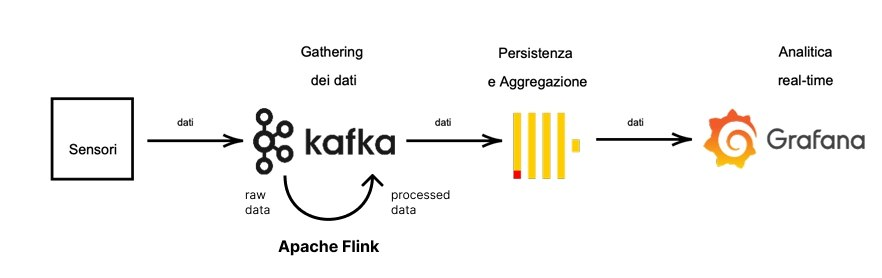
\includegraphics[width=\linewidth]{image_adr/stack.jpg}
\caption{Stack tecnologico.}
\end{figure}
\newpage
\section{Casi d'uso} \label{sec:use-case}
\subsection{Introduzione}
Di seguito sono elencati i casi d'uso individuati attraverso l'analisi del \glossterm{capitolato} e il
confronto con la \glossterm{Proponente}. Ciascuno di essi è corredato di un codice identificativo, la cui
struttura è descritta alla sezione \textit{2.3.2.4} del documento \textit{Norme di Progetto v2.0.0}. %INSERIRE RIMANDO SEZIONE CORRETTA
\subsection{Attori}
Gli attori che interagiscono con il \glossterm{sistema} sono i seguenti:
\begin{itemize}
    \item \textbf{Amministratore pubblico}: utente in grado di accedere al \glossterm{sistema} ed usufruire di tutte le sue \glossterm{funzionalità}. In particolare, può visualizzare la \glossterm{dashboard} contenente i dati provenienti dai sensori. L'applicativo richiede autenticazione;
    \item \textbf{Sensore}: dispositivo in grado di rilevare dati dall'ambiente esterno e inviare le misurazioni effettuate al \glossterm{sistema}, in modo da consentirne l'archiviazione e la successiva visualizzazione.
\end{itemize}
\clearpage
\subsection{Codice dei casi d'uso}
Ad ogni caso d'uso è associato un codice univoco definito nel seguente formato:
\begin{center}
    \textbf{UC-[Numero].[Specializzazione]}
\end{center}
Dove \textbf{Numero} è un identificativo e \textbf{Specializzazione} si riferisce ad un caso specifico
dello stesso caso d'uso.
\subsection{Elenco dei casi d'uso}
% ------------------ ISTRUZIONI PER L'USO DEI COUNTER: ------------------
% \the<nomecounter> ---> restituisce il valore ATTUALE del counter 
% \<nomecounter>number ---> INCREMENTA di 1 il counter
% \setcounter{<nomecounter>}{<numero>} ---> inizializza il counter al numero indicato. 

\newcounter{uc} %numero dello Use Case
\setcounter{uc}{-1}
\newcommand{\ucnumber}{\stepcounter{uc}\arabic{uc}}
\newcounter{specone} %primo numero del sottocaso
\setcounter{specone}{0}
\newcommand{\speconenumber}{\stepcounter{specone}\arabic{specone}}
\newcounter{spectwo} %secondo numero del sottocaso
\setcounter{spectwo}{0}
\newcommand{\spectwonumber}{\stepcounter{spectwo}\arabic{spectwo}}

\subsubsection*{UC-\ucnumber: Autenticazione} 
\addcontentsline{toc}{subsubsection}{\protect\numberline{}UC-\theuc: Autenticazione}
\begin{itemize}
    \item \textbf{Attore principale:} amministratore pubblico;
    \item \textbf{Precondizioni:} il \glossterm{sistema} è operativo e accessibile. L'amministratore pubblico è in possesso delle credenziali di accesso;
    \item \textbf{Postcondizioni:} l'amministratore pubblico ha accesso al \glossterm{sistema}.
    \item \textbf{Scenario principale:} 
        \begin{enumerate}
        \item L'amministratore pubblico avvia l'applicativo web e visualizza la pagina di login;
        \item L'amministratore pubblico digita le proprie credenziali (username e password) nei rispettivi campi di inserimento;
        \item Il sistema invia i dati inseriti dall'amministratore pubblico a \glossterm{Grafana} per la loro verifica;
        \item Le credenziali fornite vengono verificate.
        \end{enumerate}
        % immagine
    \item \textbf{\glossterm{User Story} associata:} in qualità di amministratore pubblico, desidero accedere al \glossterm{sistema} e visualizzare la pagina principale dell'applicazione web. Ciò è possibile soltanto dopo aver digitato correttamente le credenziali di accesso negli appositi campi di inserimento, presenti nella schermata di login.
    \item \textbf{Specializzazioni:} [UC-\theuc .1], [UC-\theuc .1];
    \item \textbf{Estensioni:} [UC-1].
\end{itemize}

\begin{figure}[ht!]
    \centering
        \begin{tikzpicture}
            \umlactor[x=0, y=0]{Amministratore pubblico}
            \begin{umlsystem}[x=6, y=0]{SyncCity}
                \umlusecase[x=0, y=0, width=80, name=UC-0]{UC-\theuc \\ Autenticazione}

                \umlusecase[x=0, y=-3, width=80, name=UC-1]{UC-1 \\ Visualizzazione messaggio credenziali errate}
            \end{umlsystem}
                \umlassoc{Amministratore pubblico}{UC-0}
                \umlextend{UC-1}{UC-0}
        \end{tikzpicture}
    \caption{UC-\theuc: Autenticazione.}
    \label{fig:UC-\theuc: Autenticazione}
\end{figure}

\subsubsection*{UC-\theuc .\speconenumber: Inserimento username} 
\addcontentsline{toc}{subsubsection}{\protect\numberline{}UC-\theuc .\thespecone: Inserimento username}
\begin{itemize}
    \item \textbf{Attore principale:} amministratore pubblico;
    \item \textbf{Precondizioni:} il \glossterm{sistema} è operativo e accessibile. L'amministratore pubblico è in possesso delle credenziali di accesso e sta visualizzando la pagina di login;
    \item \textbf{Postcondizioni:} lo username dell'amministratore pubblico è stato inserito nel campo corrispondente.
    \item \textbf{Scenario principale:} 
        \begin{enumerate}
        \item L'amministratore pubblico digita il proprio username nell'omonimo campo di inserimento.
        \end{enumerate}
        % immagine
    \item \textbf{\glossterm{User Story} associata:} in qualità di amministratore pubblico, desidero inserire il mio username nell'apposito campo per poter avere accesso al \glossterm{sistema}.
\end{itemize}

\subsubsection*{UC-\theuc .\speconenumber: Inserimento password} 
\addcontentsline{toc}{subsubsection}{\protect\numberline{}UC-\theuc .\thespecone: Inserimento password}
\begin{itemize}
    \item \textbf{Attore principale:} amministratore pubblico;
    \item \textbf{Precondizioni:} il \glossterm{sistema} è operativo e accessibile. L'amministratore pubblico è in possesso delle credenziali di accesso e sta visualizzando la pagina di login;
    \item \textbf{Postcondizioni:} la password dell'amministratore pubblico è stata inserita nel campo corrispondente.
    \item \textbf{Scenario principale:} 
        \begin{enumerate}
        \item L'amministratore pubblico digita la propria password nell'omonimo campo di inserimento.
        \end{enumerate}
        % immagine
    \item \textbf{\glossterm{User Story} associata:} in qualità di amministratore pubblico, desidero inserire la mia password nell'apposito campo per poter avere accesso al \glossterm{sistema}.
\end{itemize}

\begin{figure}[ht!]
    \centering
        \begin{tikzpicture}
            \umlactor[x=0, y=-1.25, inner xsep=3em, inner ysep=3em]{Amministratore pubblico}
            \begin{umlsystem}[x=7, y=0]{UC-\theuc { }Autenticazione}
                \umlusecase[x=0, y=0, width=80, name=UC-user]{UC-\theuc .1 \\ Inserimento username}

                \umlusecase[x=0, y=-2.5, width=80, name=UC-psw]{UC-\theuc .2 \\ Inserimento password}

            \end{umlsystem}
                \umlassoc{Amministratore pubblico}{UC-user}
                \umlassoc{Amministratore pubblico}{UC-psw}
        \end{tikzpicture}
    \caption{Sottocasi UC-\theuc: Autenticazione.}
    \label{fig:Sottocasi UC-\theuc: Autenticazione}
\end{figure}

\subsubsection*{UC-\ucnumber: Visualizzazione messaggio credenziali errate}
\addcontentsline{toc}{subsubsection}{\protect\numberline{}UC-\theuc: Visualizzazione messaggio credenziali errate}
\begin{itemize}
    \item \textbf{Attore principale:} amministratore pubblico;
    \item \textbf{Precondizioni:} il \glossterm{sistema} è operativo e accessibile. L'amministratore pubblico ha inserito delle credenziali di accesso errate;
    \item \textbf{Postcondizioni:} l'amministratore pubblico visualizza un messaggio di errore segnalante l'inesattezza dei dati digitati.
    \item \textbf{Scenario principale:} 
        \begin{enumerate}
        \item Il \glossterm{sistema} verifica le credenziali inserite dall'amministratore pubblico;
        \item Username o password non sono corretti, dunque viene visualizzato un messaggio di errore.
        \end{enumerate}
        % immagine
    \item \textbf{\glossterm{User Story} associata:} in qualità di amministratore pubblico, desidero essere notificato qualora l'autenticazione fallisse a causa dell'inserimento di dati errati.
\end{itemize}
\begin{figure}[ht!]
    \centering
        \begin{tikzpicture}
            \umlactor[x=0, y=0]{Amministratore pubblico}
            \begin{umlsystem}[x=6, y=0]{SyncCity}
                \umlusecase[x=0, y=0, width=80, name=UC-1]{UC-\theuc \\ Visualizzazione messaggio credenziali errate}
            \end{umlsystem}
                \umlassoc{Amministratore pubblico}{UC-1}
        \end{tikzpicture}
    \caption{UC-\theuc: Visualizzazione messaggio credenziali errate.}
    \label{fig:UC-\theuc: Visualizzazione messaggio credenziali errate}
\end{figure}

\subsubsection*{UC-\ucnumber: Visualizzazione menu \glossterm{dashboard}}
\addcontentsline{toc}{subsubsection}{\protect\numberline{}UC-\theuc: Visualizzazione menu \glossterm{dashboard}}
\begin{itemize}
    \item \textbf{Attore principale:} amministratore pubblico;
    \item \textbf{Precondizioni:} il \glossterm{sistema} è operativo e accessibile;
    \item \textbf{Postcondizioni:} l'amministratore pubblico visualizza un menu di selezione da cui
        può scegliere una specifica \glossterm{dashboard}: Sensori, Ambientale, Urbanistica o Soglie.
    \item \textbf{Scenario principale:} 
        \begin{enumerate}
        \item L'amministratore pubblico accede alla piattaforma di visualizzazione.
        \end{enumerate}
        % immagine
    \item \textbf{\glossterm{User Story} associata:} in qualità di amministratore pubblico, desidero accedere alla \glossterm{dashboard} per monitorare in tempo reale i dati raccolti dai vari sensori dislocati nella città. Questo mi permetterà di valutarne rapidamente lo stato complessivo e prendere decisioni informate e tempestive riguardo alla gestione delle risorse e all’implementazione dei servizi.
\end{itemize}
\begin{figure}[ht!]
    \centering
        \begin{tikzpicture}
            \umlactor[x=0, y=0]{Amministratore pubblico}
            \begin{umlsystem}[x=6, y=0]{SyncCity}
                \umlusecase[x=0, y=0, width=80, name=UC-0]{UC-\theuc \\ Visualizzazione menu \glossterm{dashboard}}
            \end{umlsystem}
                \umlassoc{Amministratore pubblico}{UC-0}
        \end{tikzpicture}
    \caption{UC-\theuc: Visualizzazione menu \glossterm{dashboard}.}
    \label{fig:UC-\theuc: Visualizzazione menu dashboard}
\end{figure}

\subsubsection*{UC-\ucnumber: Visualizzazione \glossterm{dashboard} sensori}
\addcontentsline{toc}{subsubsection}{\protect\numberline{}UC-\theuc: Visualizzazione \glossterm{dashboard} sensori}
\begin{itemize}
    \item \textbf{Attore principale:} amministratore pubblico;
    \item \textbf{Precondizioni:} nessuna;
    \item \textbf{Postcondizioni:} l'amministratore pubblico visualizza un pannello contenente dati relativi alle informazioni dei sensori;
    \item \textbf{Scenario principale:}
    \begin{enumerate}
    \item L'amministratore pubblico accede alla piattaforma di visualizzazione;
    \item L'amministratore pubblico seleziona la visualizzazione della \glossterm{dashboard} relativa ai sensori.
    \end{enumerate}
    \item \textbf{\glossterm{User Story} associata:} in qualità di amministratore pubblico, desidero accedere alla \glossterm{dashboard} per visualizzare la tipologia e la posizione dei sensori dislocati nella città;
    \item \textbf{Specializzazioni:} [UC-\theuc .1];
    \item \textbf{Estensioni:} [UC-7].
\end{itemize}
\begin{figure}[ht!]
    \centering
        \begin{tikzpicture}
            \umlactor[x=0, y=0]{Amministratore pubblico}
            \begin{umlsystem}[x=6, y=0]{SyncCity}
                \umlusecase[x=0, y=0, width=80, name=UC-1]{UC-\theuc \\ Visualizzazione \glossterm{dashboard} sensori}

                \umlusecase[x=0, y=-3, width=80, name=UC-7]{UC-7 \\ Visualizzazione errore nessun dato}
            \end{umlsystem}
                \umlassoc{Amministratore pubblico}{UC-1}
                \umlextend{UC-7}{UC-1}
        \end{tikzpicture}
    \caption{UC-\theuc: Visualizzazione \glossterm{dashboard} sensori.}
    \label{fig:UC-\theuc: Visualizzazione dashboard sensori}
\end{figure}
\setcounter{specone}{0}
\subsubsection*{UC-\theuc .\speconenumber: Visualizzazione pannello \glossterm{geomap} per posizione sensori}
\addcontentsline{toc}{subsubsection}{\protect\numberline{}UC-\theuc .\thespecone: Visualizzazione pannello \glossterm{geomap} per visualizzazione sensori}
\begin{itemize}
    \item \textbf{Attore principale:} amministratore pubblico;
    \item \textbf{Precondizioni:} l'amministratore pubblico ha selezionato la visualizzazione relativa al dominio dei sensori;
    \item \textbf{Postcondizioni:} l'amministratore pubblico visualizza un pannello che mostra la posizione dei sensori, in formato \glossterm{geomap};
    \item \textbf{Scenario principale:}
    \begin{enumerate}
      \item L'amministratore pubblico accede alla piattaforma di visualizzazione;
      \item L'amministratore pubblico seleziona la visualizzazione della \glossterm{dashboard} relativa ai sensori;
      \item L'amministratore pubblico seleziona la visualizzazione del pannello \glossterm{geomap} per la posizione dei sensori.
    \end{enumerate}
    \item \textbf{\glossterm{User Story} associata:} in qualità di amministratore pubblico, desidero accedere al pannello per conoscere le informazioni dei sensori dislocati nella città. La mappa deve indicare chiaramente la posizione di ciascun \glossterm{sensore} e deve essere etichettata in modo da consentire un riconoscimento immediato della tipologia di ogni sensore.
    \item \textbf{Specializzazioni:} [UC-\theuc .\thespecone .1].
\end{itemize}
\begin{figure}[ht!]
    \centering
        \begin{tikzpicture}
            \umlactor[x=0, y=0]{Amministratore pubblico}
            \begin{umlsystem}[x=6, y=0]{UC-\theuc Visualizzazione dashboard sensori}
                \umlusecase[x=0, y=0, width=100, name=UC-position]{UC-\theuc .\thespecone \\ Visualizzazione pannello \glossterm{geomap} per posizione sensori}
            \end{umlsystem}
                \umlassoc{Amministratore pubblico}{UC-position}
        \end{tikzpicture}
    \caption{UC-\theuc .\thespecone: Visualizzazione pannello \glossterm{geomap} per posizione sensori.}
    \label{fig:UC-\theuc .\thespecone: Visualizzazione pannello geomap per posizione sensori}
\end{figure}
\subsubsection*{UC-\theuc .\thespecone .\spectwonumber: Visualizzazione informazioni sensore}
\addcontentsline{toc}{subsubsection}{\protect\numberline{}UC-\theuc .\thespecone .\thespectwo: Visualizzazione informazioni sensore}
\begin{itemize}
    \item \textbf{Attore principale:} amministratore pubblico;
    \item \textbf{Precondizioni:} l'amministratore pubblico ha selezionato un sensore visualizzato nel pannello \glossterm{geomap};
    \item \textbf{Postcondizioni:} l'amministratore pubblico visualizza un popup con il nome e le coordinate geografiche di un sensore;
    \item \textbf{Scenario principale:}
    \begin{enumerate}
        \item L'amministratore pubblico accede alla piattaforma di visualizzazione;
        \item L'amministratore pubblico seleziona la visualizzazione della \glossterm{dashboard} relativa ai sensori;
        \item L'amministratore pubblico seleziona la visualizzazione del pannello \glossterm{geomap} per la posizione dei sensori;
        \item L'amministratore pubblico seleziona la visualizzazione di un sensore specifico per il nome e coordinate geografiche.
    \end{enumerate}
    \item \textbf{\glossterm{User Story} associata:} in qualità di amministratore pubblico, desidero visualizzare il popup per conoscere le informazioni di un sensore. Questo consente di identificare un dato sensore con il suo relativo nome e conoscere le sue coordinate geografiche precise.
\end{itemize}
\begin{figure}[ht!]
    \centering
        \begin{tikzpicture}
            \umlactor[x=0, y=0]{Amministratore pubblico}
            \begin{umlsystem}[x=7.35, y=0]{{UC-\theuc .\thespecone { }Visualizzazione pannello geomap per posizione sensori}}
                \umlusecase[x=0, y=0, width=100, name=UC-position]{UC-\theuc .\thespecone .\thespectwo \\ Visualizzazione informazioni sensore}
            \end{umlsystem}
                \umlassoc{Amministratore pubblico}{UC-position}
        \end{tikzpicture}
    \caption{UC-\theuc .\thespecone .\thespectwo: Visualizzazione informazioni sensore.}
    \label{fig:UC-\theuc .\thespecone .\thespectwo: Visualizzazione informazioni sensore}
\end{figure}
\subsubsection*{UC-\ucnumber: Visualizzazione \glossterm{dashboard} ambientale}
\addcontentsline{toc}{subsubsection}{\protect\numberline{}UC-\theuc: Visualizzazione \glossterm{dashboard} ambientale}
\begin{itemize}
    \item \textbf{Attore principale:} amministratore pubblico;
    \item \textbf{Precondizioni: }nessuna;
    \item \textbf{Postcondizioni:} l'amministratore pubblico visualizza una lista di pannelli
        contenenti dati relativi al dominio ambientale;
    \item \textbf{Scenario principale:} 
    \begin{enumerate}
    \item L'amministratore pubblico accede alla piattaforma di visualizzazione;
    \item L'amministratore pubblico seleziona la visualizzazione della \glossterm{dashboard} relativa al dominio ambientale.
    \end{enumerate}
    \item \textbf{\glossterm{User Story} associata:} in qualità di amministratore pubblico, desidero accedere alla \glossterm{dashboard} per monitorare il dominio ambientale, nella quale è possibile visualizzare i dati relativi a: temperatura, umidità, temperatura percepita, intensità delle precipitazioni, inquinamento dell'aria e livello dell'acqua;
    \item \textbf {Specializzazioni:} [UC-\theuc .1], [UC-\theuc .2], [UC-\theuc .3], [UC-\theuc .4], [UC-\theuc .5], [UC-\theuc .6], [UC-\theuc .7], [UC-\theuc .8], [UC-\theuc .9], [UC-\theuc .10], [UC-\theuc .11], [UC-\theuc .12], [UC-\theuc .13], [UC-\theuc .14];  
    \item \textbf{Estensioni:} [UC-7].
\end{itemize}
\begin{figure}[ht!]
    \centering
        \begin{tikzpicture}
            \umlactor[x=0, y=0]{Amministratore pubblico}
            \begin{umlsystem}[x=6, y=0]{SyncCity}
                \umlusecase[x=0, y=0, width=80, name=UC-2]{UC-\theuc \\ Visualizzazione dashboard ambientale}

                \umlusecase[x=0, y=-3, width=80, name=UC-7]{UC-7 \\ Visualizzazione errore nessun dato}
            \end{umlsystem}
                \umlassoc{Amministratore pubblico}{UC-2}
                \umlextend{UC-7}{UC-2}
        \end{tikzpicture}
    \caption{UC-\theuc: Visualizzazione \glossterm{dashboard} ambientale.}
    \label{fig:UC-\theuc: Visualizzazione dashboard ambientale}
\end{figure}
\setcounter{specone}{0}
\subsubsection*{UC-\theuc .\speconenumber: Visualizzazione pannello \glossterm{time series} per temperatura}
\addcontentsline{toc}{subsubsection}{\protect\numberline{}UC-\theuc .\thespecone: Visualizzazione pannello \glossterm{time series} per temperatura}
\begin{itemize}
    \item \textbf{Attore principale:} amministratore pubblico;
    \item \textbf{Precondizioni: }l’amministratore pubblico ha selezionato la visualizzazione
        relativa al dominio ambientale;
    \item \textbf{Postcondizioni:} l’amministratore pubblico visualizza un pannello con un grafico che mostra la temperatura, espressa in gradi Celsius (°C), in formato \glossterm{time series}.
    \item \textbf{Scenario principale}:
    \begin{enumerate}
    \item L’amministratore pubblico accede alla piattaforma di visualizzazione;
    \item L’amministratore pubblico seleziona la visualizzazione della \glossterm{dashboard} relativa al dominio ambientale;
    \item L’amministratore pubblico seleziona la visualizzazione del pannello \glossterm{time series} per la temperatura.
    \end{enumerate}
\item \textbf{\glossterm{User Story} associata:} in qualità di amministratore pubblico, desidero accedere al pannello per monitorare l'andamento della temperatura. Questo consente di semplificare la comprensione e la comparazione delle misurazioni.
\end{itemize}
\subsubsection*{UC-\theuc .\speconenumber: Visualizzazione pannello \glossterm{time series} per umidità}
\addcontentsline{toc}{subsubsection}{\protect\numberline{}UC-\theuc .\thespecone: Visualizzazione pannello \glossterm{time series} per umidità}
\begin{itemize}
    \item \textbf{Attore principale:} amministratore pubblico;
    \item \textbf{Precondizioni: }l’amministratore pubblico ha selezionato la visualizzazione
        relativa al dominio ambientale;
    \item \textbf{Postcondizioni:} l’amministratore pubblico visualizza un pannello con un grafico
        che mostra l'umidità relativa, espressa in percentuale, in formato \glossterm{time series}.
    \item \textbf{Scenario principale}:
    \begin{enumerate}
    \item L’amministratore pubblico accede alla piattaforma di visualizzazione;
    \item L’amministratore pubblico seleziona la visualizzazione della \glossterm{dashboard} relativa al dominio
        ambientale; 
    \item L’amministratore pubblico seleziona la visualizzazione del pannello \glossterm{time series} per
        l'umidità.
    \end{enumerate}
\item \textbf{\glossterm{User Story} associata:} in qualità di amministratore pubblico, desidero accedere al pannello per monitorare l'andamento dell'umidità relativa. Questo consente di semplificare la comprensione e la comparazione delle misurazioni.
\end{itemize}
\subsubsection*{UC-\theuc .\speconenumber: Visualizzazione pannello \glossterm{time series} per temperatura percepita}
\addcontentsline{toc}{subsubsection}{\protect\numberline{}UC-\theuc .\thespecone: Visualizzazione pannello \glossterm{time series} per temperatura percepita}
\begin{itemize}
    \item \textbf{Attore principale:} amministratore pubblico;
    \item \textbf{Precondizioni: }l'amministratore pubblico ha selezionato la visualizzazione
        relativa al dominio ambientale;
    \item \textbf{Postcondizioni:} l'amministratore pubblico visualizza un pannello con un grafico che mostra la temperatura, in gradi Celsius (°C), in formato \glossterm{time series} in relazione all'umidità.
    \item \textbf{Scenario principale}:
    \begin{enumerate}
    \item L’amministratore pubblico accede alla piattaforma di visualizzazione;
    \item L’amministratore pubblico seleziona la visualizzazione della \glossterm{dashboard} relativa al dominio
        ambientale; 
    \item L’amministratore pubblico seleziona la visualizzazione del pannello \glossterm{time series} per la temperatura percepita.
    \end{enumerate}
\item \textbf{\glossterm{User Story} associata:} in qualità di amministratore pubblico, desidero accedere al pannello per monitorare l'andamento della temperatura percepita. Questo consente di semplificare la comprensione e la comparazione delle misurazioni.
\end{itemize}
\subsubsection*{UC-\theuc .\speconenumber: Visualizzazione pannello \glossterm{Gauge} per temperatura media}
\addcontentsline{toc}{subsubsection}{\protect\numberline{}UC-\theuc .\thespecone: Visualizzazione pannello \glossterm{Gauge} per temperatura media}
\begin{itemize}
    \item \textbf{Attore principale:} amministratore pubblico;
    \item \textbf{Precondizioni: }l'amministratore pubblico ha selezionato la visualizzazione
        relativa al dominio ambientale;
    \item \textbf{Postcondizioni:} l'amministratore pubblico visualizza un pannello con un grafico che mostra la media della temperatura, in gradi Celsius (°C), in formato di diagramma di \glossterm{Gauge} considerando le ultime rilevazioni effettuate dai singoli sensori attivi all'interno della \glossterm{dashboard}.
    \item \textbf{Scenario principale}:
    \begin{enumerate}
    \item L’amministratore pubblico accede alla piattaforma di visualizzazione;
    \item L’amministratore pubblico seleziona la visualizzazione della \glossterm{dashboard} relativa al dominio
        ambientale; 
    \item L’amministratore pubblico seleziona la visualizzazione del pannello per la temperatura
        media.
    \end{enumerate}
\item \textbf{\glossterm{User Story} associata:} in qualità di amministratore pubblico, desidero accedere al pannello per monitorare la temperatura media. Questo consente di semplificare la comprensione e la comparazione delle misurazioni.
\end{itemize}
\subsubsection*{UC-\theuc .\speconenumber: Visualizzazione pannello \glossterm{Gauge} per umidità media}
\addcontentsline{toc}{subsubsection}{\protect\numberline{}UC-\theuc .\thespecone: Visualizzazione pannello \glossterm{Gauge} per umidità media}
\begin{itemize}
    \item \textbf{Attore principale:} amministratore pubblico;
    \item \textbf{Precondizioni: }l'amministratore pubblico ha selezionato la visualizzazione
        relativa al dominio ambientale;
    \item \textbf{Postcondizioni:} l'amministratore pubblico visualizza un pannello con un grafico che mostra la media dell'umidità, in gradi Celsius (°C), in formato di diagramma di \glossterm{Gauge} considerando le ultime rilevazioni effettuate dai singoli sensori attivi all'interno della \glossterm{dashboard}.
    \item \textbf{Scenario principale}:
    \begin{enumerate}
    \item L’amministratore pubblico accede alla piattaforma di visualizzazione;
    \item L’amministratore pubblico seleziona la visualizzazione della \glossterm{dashboard} relativa al dominio
        ambientale; 
    \item L’amministratore pubblico seleziona la visualizzazione del pannello per l'umidità media.
    \end{enumerate}
\item \textbf{\glossterm{User Story} associata:} in qualità di amministratore pubblico, desidero accedere al pannello per monitorare l'umidità media. Questo consente di semplificare la comprensione e la comparazione delle misurazioni.
\end{itemize}
\subsubsection*{UC-\theuc .\speconenumber: Visualizzazione pannello \glossterm{Gauge} per temperatura percepita media}
\addcontentsline{toc}{subsubsection}{\protect\numberline{}UC-\theuc .\thespecone: Visualizzazione pannello \glossterm{Gauge} per temperatura percepita media}
\begin{itemize}
    \item \textbf{Attore principale:} amministratore pubblico;
    \item \textbf{Precondizioni: }l'amministratore pubblico ha selezionato la visualizzazione
        relativa al dominio ambientale;
    \item \textbf{Postcondizioni:} l'amministratore pubblico visualizza un pannello con un grafico che mostra la media della temperatura percepita, in gradi Celsius (°C), in formato di diagramma di \glossterm{Gauge} considerando le ultime rilevazioni effettuate dalle coppie di sensori temperatura-umidità attivi all'interno della \glossterm{dashboard}.
    \item \textbf{Scenario principale}:
    \begin{enumerate}
    \item L’amministratore pubblico accede alla piattaforma di visualizzazione;
    \item L’amministratore pubblico seleziona la visualizzazione della \glossterm{dashboard} relativa al dominio
        ambientale; 
    \item L’amministratore pubblico seleziona la visualizzazione del pannello per la temperatura percepita
        media.
    \end{enumerate}
\item \textbf{\glossterm{User Story} associata:} in qualità di amministratore pubblico, desidero accedere al pannello per monitorare la temperatura percepita media. Questo consente di semplificare la comprensione e la comparazione delle misurazioni.
\end{itemize}
\subsubsection*{UC-\theuc .\speconenumber: Visualizzazione pannello con grafico a barre per valori statistici di temperatura}
\addcontentsline{toc}{subsubsection}{\protect\numberline{}UC-\theuc .\thespecone: Visualizzazione pannello \glossterm{bar chart} per valori statistici di temperatura}
\begin{itemize}
    \item \textbf{Attore principale:} amministratore pubblico;
    \item \textbf{Precondizioni:} l'amministratore pubblico ha selezionato la visualizzazione
        relativa al dominio ambientale;
    \item \textbf{Postcondizioni:} l'amministratore pubblico visualizza un pannello con un grafico che mostra i valori statistici di temperatura, in gradi Celsius (°C), in formato di diagramma a barre considerando per ciascun \glossterm{sensore} attivo nell'intervallo di tempo all'interno della \glossterm{dashboard}.
    \item \textbf{Scenario principale}:
    \begin{enumerate}
    \item L'amministratore pubblico accede alla piattaforma di visualizzazione;
    \item L'amministratore pubblico seleziona la visualizzazione della \glossterm{dashboard} relativa al dominio
        ambientale; 
    \item L'amministratore pubblico seleziona la visualizzazione del pannello per i valori statistici di temperatura.
    \end{enumerate}
\item \textbf{\glossterm{User Story} associata:} in qualità di amministratore pubblico, desidero accedere al pannello per monitorare i valori statistici di temperatura in ogni zona della città. Questo pannello consente di comprendere lo stato attuale climatico della zona d'interesse con maggiore facilità.
\end{itemize}
\subsubsection*{UC-\theuc .\speconenumber: Visualizzazione pannello con grafico a barre per valori statistici di temperatura percepita}
\addcontentsline{toc}{subsubsection}{\protect\numberline{}UC-\theuc .\thespecone: Visualizzazione pannello con grafico a barre per valori statistici di temperatura percepita}
\begin{itemize}
    \item \textbf{Attore principale:} amministratore pubblico;
    \item \textbf{Precondizioni: }l'amministratore pubblico ha selezionato la visualizzazione
        relativa al dominio ambientale;
    \item \textbf{Postcondizioni:} l'amministratore pubblico visualizza un pannello con un grafico che mostra i valori statistici di temperatura percepita, in gradi Celsius (°C), in formato di diagramma a barre considerando ciascuna coppia di valori di temperatura e umidità per ogni rispettivo \glossterm{sensore} attivo nell'intervallo di tempo all'interno della \glossterm{dashboard}.
    \item \textbf{Scenario principale}:
    \begin{enumerate}
    \item L'amministratore pubblico accede alla piattaforma di visualizzazione;
    \item L'amministratore pubblico seleziona la visualizzazione della \glossterm{dashboard} relativa al dominio
        ambientale; 
    \item L'amministratore pubblico seleziona la visualizzazione del pannello per valori statistici di temperatura percepita.
        media.
    \end{enumerate}
\item \textbf{\glossterm{User Story} associata:} in qualità di amministratore pubblico, desidero accedere al pannello per monitorare i valori statistici di temperatura percepita in ogni zona d'interesse della città.
\end{itemize}
\subsubsection*{UC-\theuc .\speconenumber: Visualizzazione pannello \glossterm{time series} per precipitazioni}
\addcontentsline{toc}{subsubsection}{\protect\numberline{}UC-\theuc .\thespecone: Visualizzazione pannello \glossterm{time series} per precipitazioni}
\begin{itemize}
    \item \textbf{Attore principale:} amministratore pubblico;
    \item \textbf{Precondizioni: }l'amministratore pubblico ha selezionato la visualizzazione
        relativa al dominio ambientale;
    \item \textbf{Postcondizioni:} l'amministratore pubblico visualizza un pannello con un grafico
        che mostra l'intensità delle precipitazioni, espressa in millimetri orari (mm/h), in formato \glossterm{time series}.
    \item \textbf{Scenario principale}:
    \begin{enumerate}
    \item L'amministratore pubblico accede alla piattaforma di visualizzazione;
    \item L'amministratore pubblico seleziona la visualizzazione della \glossterm{dashboard} relativa al dominio
        ambientale; 
    \item L'amministratore pubblico seleziona la visualizzazione del pannello \glossterm{time series} per le precipitazioni.
    \end{enumerate}
\item \textbf{\glossterm{User Story} associata:} in qualità di amministratore pubblico, desidero accedere al pannello per monitorare l'intensità delle precipitazioni. Questo consente di semplificare la comprensione e la comparazione delle misurazioni.
\end{itemize}
\subsubsection*{UC-\theuc .\speconenumber: Visualizzazione pannello \glossterm{time series} per inquinamento dell'aria}
\addcontentsline{toc}{subsubsection}{\protect\numberline{}UC-\theuc .\thespecone: Visualizzazione pannello \glossterm{time series} per inquinamento dell'aria}
\begin{itemize}
    \item \textbf{Attore principale:} amministratore pubblico;
    \item \textbf{Precondizioni:} l'amministratore pubblico ha selezionato la visualizzazione
        relativa al dominio ambientale;
    \item \textbf{Postcondizioni:} l'amministratore pubblico visualizza un pannello con un grafico
        che mostra la quantità di polveri sottili presenti nell'aria, espressa in microgrammi per metro cubo (µg / $\mbox{m}^{\mbox{3}}$), in formato \glossterm{time series}.
    \item \textbf{Scenario principale}:
    \begin{enumerate}
    \item L'amministratore pubblico accede alla piattaforma di visualizzazione;
    \item L'amministratore pubblico seleziona la visualizzazione della \glossterm{dashboard} relativa al dominio
        ambientale; 
    \item L'amministratore pubblico seleziona la visualizzazione del pannello \glossterm{time series} per l'inquinamento dell'aria.
    \end{enumerate}
\item \textbf{\glossterm{User Story} associata:} in qualità di amministratore pubblico, desidero accedere al
        pannello per monitorare il livello di polveri sottili presenti nell'aria. Questo consente di semplificare la comprensione e la comparazione delle misurazioni.
\end{itemize}
\subsubsection*{UC-\theuc .\speconenumber: Visualizzazione pannello \glossterm{time series} per livello di acqua}
\addcontentsline{toc}{subsubsection}{\protect\numberline{}UC-\theuc .\thespecone: Visualizzazione pannello \glossterm{time series} per livello di acqua}
\begin{itemize}
    \item \textbf{Attore principale:} amministratore pubblico;
    \item \textbf{Precondizioni:} l'amministratore pubblico ha selezionato la visualizzazione
        relativa al dominio ambientale;
    \item \textbf{Postcondizioni:} l'amministratore pubblico visualizza un pannello con un grafico che mostra le misurazioni relative al livello dell'acqua, espresse in percentuale, in formato \glossterm{time series}.
    \item \textbf{Scenario principale}:
    \begin{enumerate}
    \item L'amministratore pubblico accede alla piattaforma di visualizzazione;
    \item L'amministratore pubblico seleziona la visualizzazione della \glossterm{dashboard} relativa al dominio
        ambientale; 
    \item L'amministratore pubblico seleziona la visualizzazione del pannello per il livello dell'acqua.
    \end{enumerate}
\item \textbf{\glossterm{User Story} associata:} in qualità di amministratore pubblico, desidero accedere al
        pannello per monitorare il livello dell'acqua. Questo consente di semplificare la comprensione e la comparazione delle misurazioni.
\end{itemize}
\subsubsection*{UC-\theuc .\speconenumber: Visualizzazione pannello \glossterm{Gauge} per intensità attuale delle precipitazioni}
\addcontentsline{toc}{subsubsection}{\protect\numberline{}UC-\theuc .\thespecone: Visualizzazione pannello \glossterm{Gauge} per intensità attuale delle precipitazioni}
\begin{itemize}
    \item \textbf{Attore principale:} amministratore pubblico;
    \item \textbf{Precondizioni:} l'amministratore pubblico ha selezionato la visualizzazione
        relativa al dominio ambientale;
    \item \textbf{Postcondizioni:} l'amministratore pubblico visualizza un pannello con un grafico che mostra l'intensità attuale delle precipitazioni, in gradi millimetri orari (mm/h), in formato di diagramma di \glossterm{Gauge} considerando le ultime rilevazioni effettuate dai singoli sensori attivi all'interno della \glossterm{dashboard}.
    \item \textbf{Scenario principale}:
    \begin{enumerate}
    \item L'amministratore pubblico accede alla piattaforma di visualizzazione;
    \item L'amministratore pubblico seleziona la visualizzazione della \glossterm{dashboard} relativa al dominio
        ambientale; 
    \item L'amministratore pubblico seleziona la visualizzazione del pannello per l'intensità attuale delle precipitazioni.
    \end{enumerate}
\item \textbf{\glossterm{User Story} associata:} in qualità di amministratore pubblico, desidero accedere al pannello per monitorare l'intensità attuale delle precipitazioni. Questo consente di semplificare la comprensione e la comparazione delle misurazioni.
\end{itemize}
\subsubsection*{UC-\theuc .\speconenumber: Visualizzazione pannello \glossterm{Gauge} per inquinamento attuale dell'aria}
\addcontentsline{toc}{subsubsection}{\protect\numberline{}UC-\theuc .\thespecone: Visualizzazione pannello \glossterm{Gauge} per inquinamento attuale dell'aria}
\begin{itemize}
    \item \textbf{Attore principale:} amministratore pubblico;
    \item \textbf{Precondizioni:} l'amministratore pubblico ha selezionato la visualizzazione
        relativa al dominio ambientale;
    \item \textbf{Postcondizioni:} l'amministratore pubblico visualizza un pannello con un grafico che mostra l'inquinamento attuale dell'aria, in microgrammi per metro cubo (µg / $\mbox{m}^{\mbox{3}}$), in formato di diagramma di \glossterm{Gauge} considerando le ultime rilevazioni effettuate dai singoli sensori attivi all'interno della \glossterm{dashboard}.
    \item \textbf{Scenario principale}:
    \begin{enumerate}
    \item L'amministratore pubblico accede alla piattaforma di visualizzazione;
    \item L'amministratore pubblico seleziona la visualizzazione della \glossterm{dashboard} relativa al dominio
        ambientale; 
    \item L'amministratore pubblico seleziona la visualizzazione del pannello per l'inquinamento attuale dell'aria.
    \end{enumerate}
\item \textbf{\glossterm{User Story} associata:} in qualità di amministratore pubblico, desidero accedere al pannello per monitorare l'inquinamento attuale dell'aria. Questo consente di semplificare la comprensione e la comparazione delle misurazioni.
\end{itemize}
\subsubsection*{UC-\theuc .\speconenumber: Visualizzazione pannello \glossterm{Gauge} per livello attuale dell'acqua}
\addcontentsline{toc}{subsubsection}{\protect\numberline{}UC-\theuc .\thespecone: Visualizzazione pannello \glossterm{Gauge} per livello attuale dell'acqua}
\begin{itemize}
    \item \textbf{Attore principale:} amministratore pubblico;
    \item \textbf{Precondizioni:} l'amministratore pubblico ha selezionato la visualizzazione
        relativa al dominio ambientale;
    \item \textbf{Postcondizioni:} l'amministratore pubblico visualizza un pannello con un grafico che mostra il livello attuale dell'acqua, in percentuale, in formato di diagramma di \glossterm{Gauge} considerando le ultime rilevazioni effettuate dai singoli sensori attivi all'interno della \glossterm{dashboard}.
    \item \textbf{Scenario principale}:
    \begin{enumerate}
    \item L'amministratore pubblico accede alla piattaforma di visualizzazione;
    \item L'amministratore pubblico seleziona la visualizzazione della \glossterm{dashboard} relativa al dominio
        ambientale; 
    \item L'amministratore pubblico seleziona la visualizzazione del pannello per il livello attuale dell'acqua.
    \end{enumerate}
\item \textbf{\glossterm{User Story} associata:} in qualità di amministratore pubblico, desidero accedere al pannello per monitorare il livello attuale dell'acqua. Questo consente di semplificare la comprensione e la comparazione delle misurazioni.
\end{itemize}
\begin{figure}[ht!]
    \centering
        \begin{tikzpicture}
            \umlactor[x=0, y=-7.5, inner xsep=3em, inner ysep=3em]{Amministratore pubblico}
            \begin{umlsystem}[x=9, y=0]{UC-\theuc { }Visualizzazione dashboard ambientale}
                \umlusecase[x=0, y=0, width=100, name=UC-temp]{UC-\theuc.1 \\ Visualizzazione pannello \glossterm{time series} per temperatura}

                \umlusecase[x=0, y=-2.5, width=100, name=UC-humid]{UC-\theuc.2 \\ Visualizzazione pannello \glossterm{time series} per umidità}

                \umlusecase[x=0, y=-5, width=100, name=UC-temp-perc]{UC-\theuc.3 \\ Visualizzazione pannello \glossterm{time series} per temperatura percepita}

                \umlusecase[x=0, y=-7.5, width=100, name=UC-temp-avg]{UC-\theuc.4 \\ Visualizzazione pannello \glossterm{Gauge} per temperatura media}

                \umlusecase[x=0, y=-10, width=100, name=UC-humid-avg]{UC-\theuc.5 \\ Visualizzazione pannello \glossterm{Gauge} per umidità media}

                \umlusecase[x=0, y=-12.5, width=100, name=UC-heat-avg]{UC-\theuc.6 \\ Visualizzazione pannello \glossterm{Gauge} per temperatura percepita media}

                \umlusecase[x=0, y=-15, width=100, name=UC-temp-stat]{UC-\theuc.7 \\ Visualizzazione pannello \glossterm{bar chart} per statistiche di temperatura}
            \end{umlsystem}
                \umlassoc{Amministratore pubblico}{UC-temp}
                \umlassoc{Amministratore pubblico}{UC-humid}
                \umlassoc{Amministratore pubblico}{UC-temp-perc}
                \umlassoc{Amministratore pubblico}{UC-temp-avg}
                \umlassoc{Amministratore pubblico}{UC-humid-avg}
                \umlassoc{Amministratore pubblico}{UC-heat-avg}
                \umlassoc{Amministratore pubblico}{UC-temp-stat}
        \end{tikzpicture}
    \caption{Prima parte sottocasi UC-\theuc: Visualizzazione \glossterm{dashboard} ambientale.}
    \label{fig:Prima parte sottocasi UC-\theuc: Visualizzazione dashboard ambientale}
\end{figure}

\begin{figure}[ht!]
    \centering
        \begin{tikzpicture}
            \umlactor[x=0, y=-7.65, inner xsep=3em, inner ysep=3em]{Amministratore pubblico}
            \begin{umlsystem}[x=9, y=0]{UC-\theuc { }Visualizzazione dashboard ambientale}
                \umlusecase[x=0, y=0, width=100, name=UC-heat-stat]{UC-\theuc.8 \\ Visualizzazione pannello \glossterm{bar chart} per statistiche di temperatura percepita}

                \umlusecase[x=0, y=-2.75, width=100, name=UC-rain]{UC-\theuc.9 \\ Visualizzazione pannello \glossterm{time series} per precipitazioni}

                \umlusecase[x=0, y=-5.2, width=100, name=UC-pollut]{UC-\theuc.10 \\ Visualizzazione pannello \glossterm{time series} per inquinamento dell'aria}

                \umlusecase[x=0, y=-7.65, width=100, name=UC-water]{UC-\theuc.11 \\ Visualizzazione pannello \glossterm{time series} per livello di acqua}

                \umlusecase[x=0, y=-10.4, width=100, name=UC-rain-act]{UC-\theuc.12 \\ Visualizzazione pannello \glossterm{Gauge} per intensità attuale delle precipitazioni}

                \umlusecase[x=0, y=-13.1, width=100, name=UC-pollut-act]{UC-\theuc.13 \\ Visualizzazione pannello \glossterm{Gauge} per inquinamento attuale dell'aria}

                \umlusecase[x=0, y=-15.55, width=100, name=UC-water-act]{UC-\theuc.14 \\ Visualizzazione pannello \glossterm{Gauge} per livello attuale dell'acqua}
            \end{umlsystem}
                \umlassoc{Amministratore pubblico}{UC-heat-stat}
                \umlassoc{Amministratore pubblico}{UC-rain}
                \umlassoc{Amministratore pubblico}{UC-pollut}
                \umlassoc{Amministratore pubblico}{UC-water}
                \umlassoc{Amministratore pubblico}{UC-rain-act}
                \umlassoc{Amministratore pubblico}{UC-pollut-act}
                \umlassoc{Amministratore pubblico}{UC-water-act}
        \end{tikzpicture}
    \caption{Seconda parte sottocasi UC-\theuc: Visualizzazione \glossterm{dashboard} ambientale.}
    \label{fig:Seconda parte sottocasi UC-\theuc: Visualizzazione dashboard ambientale}
\end{figure}
\clearpage
\newpage
\subsubsection*{UC-\ucnumber: Visualizzazione \glossterm{dashboard} urbanistica}
\addcontentsline{toc}{subsubsection}{\protect\numberline{}UC-\theuc: Visualizzazione \glossterm{dashboard} urbanistica}
\begin{itemize}
    \item \textbf{Attore principale:} amministratore pubblico;
    \item \textbf{Precondizioni: }nessuna;
    \item \textbf{Postcondizioni:} l'amministratore pubblico visualizza una lista di pannelli
        contenenti dati relativi al dominio urbanistico;
    \item \textbf{Scenario principale:} 
    \begin{enumerate}
    \item L'amministratore pubblico accede alla piattaforma di visualizzazione;
    \item L'amministratore pubblico seleziona la visualizzazione della \glossterm{dashboard} relativa al dominio urbanistico.
    \end{enumerate}
    \item \textbf{\glossterm{User Story} associata:} in qualità di amministratore pubblico, desidero accedere alla \glossterm{dashboard} per monitorare il dominio urbanistico, nella quale è possibile visualizzare i dati relativi a: disponibilità e informazioni parcheggi, guasti elettrici, riempimento delle isole ecologiche e disponibilità e informazioni delle colonnine di ricarica;
    \item \textbf {Specializzazioni:} [UC-\theuc .1], [UC-\theuc .2], [UC-\theuc .3], [UC-\theuc .4], [UC-\theuc .5], [UC-\theuc .6], [UC-\theuc .7], [UC-\theuc .8], [UC-\theuc .9], [UC-\theuc .10], [UC-\theuc .11], [UC-\theuc .12];
    \item \textbf{Estensioni:} [UC-7].
\end{itemize}
\begin{figure}[ht!]
    \centering
        \begin{tikzpicture}
            \umlactor[x=0, y=0]{Amministratore pubblico}
            \begin{umlsystem}[x=6, y=0]{SyncCity}
                \umlusecase[x=0, y=0, width=80, name=UC-3]{UC-\theuc \\ Visualizzazione dashboard urbanistica}

                \umlusecase[x=0, y=-3, width=80, name=UC-7]{UC-7 \\ Visualizzazione errore nessun dato}
            \end{umlsystem}
                \umlassoc{Amministratore pubblico}{UC-3}
                \umlextend{UC-7}{UC-3}
        \end{tikzpicture}
    \caption{UC-\theuc: Visualizzazione \glossterm{dashboard} urbanistica.}
    \label{fig:UC-\theuc: Visualizzazione dashboard urbanistica}
\end{figure}
\setcounter{specone}{0}
\subsubsection*{UC-\theuc .\speconenumber: Visualizzazione pannello \glossterm{geomap} per disponibilità parcheggi}
\addcontentsline{toc}{subsubsection}{\protect\numberline{}UC-\theuc .\thespecone: Visualizzazione pannello
\glossterm{geomap} per disponibilità parcheggi}
\begin{itemize}
    \item \textbf{Attore principale:} amministratore pubblico;
    \item \textbf{Precondizioni:} l'amministratore pubblico ha selezionato la visualizzazione
        relativa al dominio urbanistico.
    \item \textbf{Postcondizioni:} l'amministratore pubblico visualizza un pannello che mostra lo
        stato di occupazione dei parcheggi, in formato \glossterm{geomap};
    \item \textbf{Scenario principale:} 
    \begin{enumerate}
    \item L'amministratore pubblico accede alla piattaforma di visualizzazione;
    \item L'amministratore pubblico seleziona la visualizzazione della \glossterm{dashboard} relativa al dominio
        urbanistico;
    \item L'amministratore pubblico seleziona la visualizzazione del pannello \glossterm{geomap} per lo stato di occupazione dei parcheggi.
    \end{enumerate}
    \item \textbf{\glossterm{User Story} associata:} in qualità di amministratore pubblico, desidero accedere al pannello per monitorare lo stato di disponibilità dei singoli parcheggi. Questo consente di semplificare la comprensione e la comparazione delle misurazioni.
\end{itemize}
\subsubsection*{UC-\theuc .\speconenumber: Visualizzazione pannello tabellare per informazioni sui parcheggi}
\addcontentsline{toc}{subsubsection}{\protect\numberline{}UC-\theuc .\thespecone: Visualizzazione pannello
tabellare per informazioni sui parcheggi}
\begin{itemize}
    \item \textbf{Attore principale:} amministratore pubblico;
    \item \textbf{Precondizioni:} l'amministratore pubblico ha selezionato la visualizzazione
        relativa al dominio urbanistico.
    \item \textbf{Postcondizioni:} l'amministratore pubblico visualizza un pannello che mostra le informazioni riguardanti i parcheggi, in formato tabellare;
    \item \textbf{Scenario principale:} 
    \begin{enumerate}
    \item L'amministratore pubblico accede alla piattaforma di visualizzazione;
    \item L'amministratore pubblico seleziona la visualizzazione della \glossterm{dashboard} relativa al dominio
        urbanistico;
    \item L'amministratore pubblico seleziona la visualizzazione del pannello tabellare per le informazioni riguardanti i parcheggi.
    \end{enumerate}
    \item \textbf{\glossterm{User Story} associata:} in qualità di amministratore pubblico, desidero accedere al pannello per monitorare lo stato dei singoli parcheggi. Questo consente di semplificare la comprensione e la comparazione delle misurazioni.
\end{itemize}
\subsubsection*{UC-\theuc .\speconenumber: Visualizzazione pannello in formato di registro per notifiche pagamento parcheggi}
\addcontentsline{toc}{subsubsection}{\protect\numberline{}UC-\theuc .\thespecone: Visualizzazione pannello in formato di registro per notifiche pagamento parcheggi}
\begin{itemize}
    \item \textbf{Attore principale:} amministratore pubblico;
    \item \textbf{Precondizioni:} l'amministratore pubblico ha selezionato la visualizzazione
        relativa al dominio urbanistico.
    \item \textbf{Postcondizioni:} l'amministratore pubblico visualizza un pannello che mostra le notifiche di pagamento relative al parcheggio.
        contenenti dati relativi al dominio urbanistico;
    \item \textbf{Scenario principale:} 
    \begin{enumerate}
    \item L'amministratore pubblico accede alla piattaforma di visualizzazione;
    \item L'amministratore pubblico seleziona la visualizzazione della \glossterm{dashboard} relativa al dominio urbanistico;
    \item L'amministratore pubblico seleziona la visualizzazione del pannello in formato di registro per le notifiche di pagamento dei parcheggi.
    \end{enumerate}
    \item \textbf{\glossterm{User Story} associata:} in qualità di amministratore pubblico, desidero accedere al pannello per monitorare i pagamenti delle soste nei parcheggi. Questo consente di semplificare la comprensione e la comparazione delle misurazioni.
\end{itemize}
\subsubsection*{UC-\theuc .\speconenumber: Visualizzazione pannello \glossterm{geomap} per guasti elettrici}
\addcontentsline{toc}{subsubsection}{\protect\numberline{}UC-\theuc .\thespecone: Visualizzazione pannello
\glossterm{geomap} per guasti elettrici}
\begin{itemize}
    \item \textbf{Attore principale:} amministratore pubblico;
    \item \textbf{Precondizioni:} l'amministratore pubblico ha selezionato la visualizzazione
        relativa al dominio urbanistico.
    \item \textbf{Postcondizioni:} l'amministratore pubblico visualizza un pannello che mostra i
        guasti sulla rete elettrica in formato \glossterm{geomap};
    \item \textbf{Scenario principale:} 
    \begin{enumerate}
    \item L'amministratore pubblico accede alla piattaforma di visualizzazione;
    \item L'amministratore pubblico seleziona la visualizzazione della \glossterm{dashboard} relativa al dominio urbanistico;
    \item L'amministratore pubblico seleziona la visualizzazione del pannello \glossterm{geomap} per i guasti.
    \end{enumerate}
    \item \textbf{\glossterm{User Story} associata:} in qualità di amministratore pubblico, desidero accedere al pannello per monitorare lo stato della fornitura elettrica. Questo consente di semplificare la comprensione e la comparazione delle misurazioni.
\end{itemize}
\subsubsection*{UC-\theuc .\speconenumber: Visualizzazione pannello \glossterm{time series} per riempimento isole ecologiche}
\addcontentsline{toc}{subsubsection}{\protect\numberline{}UC-\theuc .\thespecone: Visualizzazione pannello \glossterm{time series} per stato riempimento isole ecologiche}
\begin{itemize}
    \item \textbf{Attore principale:} amministratore pubblico;
    \item \textbf{Precondizioni:} l'amministratore pubblico ha selezionato la visualizzazione
        relativa al dominio urbanistico.
    \item \textbf{Postcondizioni:} l'amministratore pubblico visualizza un pannello che mostra la percentuale di riempimento dei conferitori, in formato \glossterm{time series};
    \item \textbf{Scenario principale:} 
    \begin{enumerate}
    \item L'amministratore pubblico accede alla piattaforma di visualizzazione;
    \item L'amministratore pubblico seleziona la visualizzazione della \glossterm{dashboard} relativa al dominio urbanistico;
    \item L'amministratore pubblico seleziona la visualizzazione del pannello \glossterm{time series} per lo stato di riempimento dei conferitori delle isole ecologiche.
    \end{enumerate}
    \item \textbf{\glossterm{User Story} associata:} in qualità di amministratore pubblico, desidero accedere al pannello per monitorare il livello di riempimento dei conferitori presenti nelle isole ecologiche. Questo consente di semplificare la comprensione e la comparazione delle misurazioni.
\end{itemize}
\subsubsection*{UC-\theuc .\speconenumber: Visualizzazione pannello \glossterm{geomap} per disponibilità colonnine di ricarica}
\addcontentsline{toc}{subsubsection}{\protect\numberline{}UC-\theuc .\thespecone: Visualizzazione pannello
\glossterm{geomap} per disponibilità colonnine di ricarica}
\begin{itemize}
    \item \textbf{Attore principale:} amministratore pubblico;
    \item \textbf{Precondizioni:} l'amministratore pubblico ha selezionato la visualizzazione
        relativa al dominio urbanistico.
    \item \textbf{Postcondizioni:} l'amministratore pubblico visualizza un pannello che mostra lo
        stato di occupazione delle colonnine di ricarica, in formato \glossterm{geomap};
    \item \textbf{Scenario principale:} 
    \begin{enumerate}
    \item L'amministratore pubblico accede alla piattaforma di visualizzazione;
    \item L'amministratore pubblico seleziona la visualizzazione della \glossterm{dashboard} relativa al dominio urbanistico;
    \item L'amministratore pubblico seleziona la visualizzazione del pannello \glossterm{geomap} per la disponibilità delle colonnine di ricarica.
    \end{enumerate}
    \item \textbf{\glossterm{User Story} associata:} in qualità di amministratore pubblico, desidero accedere al pannello per monitorare la disponibilità delle colonnine di ricarica. Questo consente di semplificare la comprensione e la comparazione delle misurazioni.
\end{itemize}
\subsubsection*{UC-\theuc .\speconenumber: Visualizzazione pannello tabellare per informazioni su colonnine di ricarica}
\addcontentsline{toc}{subsubsection}{\protect\numberline{}UC-\theuc .\thespecone: Visualizzazione pannello
tabellare per disponibilità colonnine di ricarica}
\begin{itemize}
    \item \textbf{Attore principale:} amministratore pubblico;
    \item \textbf{Precondizioni:} l'amministratore pubblico ha selezionato la visualizzazione
        relativa al dominio urbanistico.
    \item \textbf{Postcondizioni:} l'amministratore pubblico visualizza un pannello che mostra informazioni riguardanti le colonnine di ricarica, in formato tabellare;
    \item \textbf{Scenario principale:} 
    \begin{enumerate}
    \item L'amministratore pubblico accede alla piattaforma di visualizzazione;
    \item L'amministratore pubblico seleziona la visualizzazione della \glossterm{dashboard} relativa al dominio urbanistico;
    \item L'amministratore pubblico seleziona la visualizzazione del pannello in formato tabellare per informazioni riguardanti le colonnine di ricarica.
    \end{enumerate}
    \item \textbf{\glossterm{User Story} associata:} in qualità di amministratore pubblico, desidero accedere al pannello per monitorare le colonnine di ricarica. Questo consente di semplificare la comprensione e la comparazione delle misurazioni.
\end{itemize}
\subsubsection*{UC-\theuc .\speconenumber: Visualizzazione pannello \glossterm{time series} per consumi colonnine di ricarica}
\addcontentsline{toc}{subsubsection}{\protect\numberline{}UC-\theuc .\thespecone: Visualizzazione pannello \glossterm{time series} per consumi colonnine di ricarica}
\begin{itemize}
    \item \textbf{Attore principale:} amministratore pubblico;
    \item \textbf{Precondizioni:} l’amministratore pubblico ha selezionato la visualizzazione
        relativa al dominio urbanistico.
    \item \textbf{Postcondizioni:} l'amministratore pubblico visualizza un pannello che mostra i consumi di elettricità per la ricarica dei veicoli elettrici. Tali dati sono espressi in kilowattora (kWh) e rappresentati in formato \glossterm{time series};
    \item \textbf{Scenario principale:} 
    \begin{enumerate}
    \item L’amministratore pubblico accede alla piattaforma di visualizzazione;
    \item L’amministratore pubblico seleziona la visualizzazione della \glossterm{dashboard} relativa al dominio urbanistico;
    \item L’amministratore pubblico seleziona la visualizzazione del pannello \glossterm{time series} per l'erogazione di corrente elettrica dalle colonnine di ricarica.
    \end{enumerate}
    \item \textbf{\glossterm{User Story} associata:} in qualità di amministratore pubblico, desidero accedere al pannello per monitorare i consumi delle colonnine di ricarica. Questo consente di semplificare la comprensione e la comparazione delle misurazioni.
\end{itemize}
\subsubsection*{UC-\theuc .\speconenumber: Visualizzazione pannello in formato di registro per notifiche pagamento colonnine di ricarica}
\addcontentsline{toc}{subsubsection}{\protect\numberline{}UC-\theuc .\thespecone: Visualizzazione pannello in formato di registro per notifiche pagamento colonnine di ricarica}
\begin{itemize}
    \item \textbf{Attore principale:} amministratore pubblico;
    \item \textbf{Precondizioni:} l’amministratore pubblico ha selezionato la visualizzazione
        relativa al dominio urbanistico.
    \item \textbf{Postcondizioni:} l'amministratore pubblico visualizza un pannello che mostra le notifiche di pagamento delle colonnine di ricarica;
    \item \textbf{Scenario principale:} 
    \begin{enumerate}
    \item L’amministratore pubblico accede alla piattaforma di visualizzazione;
    \item L’amministratore pubblico seleziona la visualizzazione della \glossterm{dashboard} relativa al dominio urbanistico;
    \item L’amministratore pubblico seleziona la visualizzazione del pannello in formato di registro per le notifiche di pagamento delle colonnine di ricarica.
    \end{enumerate}
    \item \textbf{\glossterm{User Story} associata:} in qualità di amministratore pubblico, desidero accedere al pannello per monitorare lo stato dei pagamenti delle ricariche di veicoli elettrici effettuate grazie alle apposite colonnine. Questo consente di semplificare la comprensione e la comparazione delle misurazioni.
\end{itemize}
\subsubsection*{UC-\theuc .\speconenumber: Visualizzazione pannello \glossterm{Gauge} per dati pagamento parcheggio}
\addcontentsline{toc}{subsubsection}{\protect\numberline{}UC-\theuc .\thespecone: Visualizzazione pannello \glossterm{Gauge} per dati pagamento parcheggio}
\begin{itemize}
    \item \textbf{Attore principale:} amministratore pubblico;
    \item \textbf{Precondizioni:} l’amministratore pubblico ha selezionato la visualizzazione
        relativa al dominio urbanistico.
    \item \textbf{Postcondizioni:} l'amministratore pubblico visualizza un pannello che mostra i valori statistici dei pagamenti dei parcheggi;
    \item \textbf{Scenario principale:} 
    \begin{enumerate}
    \item L’amministratore pubblico accede alla piattaforma di visualizzazione;
    \item L’amministratore pubblico seleziona la visualizzazione della \glossterm{dashboard} relativa al dominio urbanistico;
    \item L’amministratore pubblico seleziona la visualizzazione del pannello \glossterm{Gauge} per le
        notifiche di pagamento dei parcheggi.
    \end{enumerate}
    \item \textbf{\glossterm{User Story} associata:} in qualità di amministratore pubblico, desidero accedere al
        pannello per monitorare lo stato dei pagamenti dei parcheggi. Questo consente di semplificare la comprensione e la comparazione delle misurazioni.
\end{itemize}
\subsubsection*{UC-\theuc .\speconenumber: Visualizzazione pannello \glossterm{Gauge} per dati pagamento di colonnine di ricarica}
\addcontentsline{toc}{subsubsection}{\protect\numberline{}UC-\theuc .\thespecone: Visualizzazione pannello \glossterm{Gauge} per dati pagamento di colonnine di ricarica}
\begin{itemize}
    \item \textbf{Attore principale:} amministratore pubblico;
    \item \textbf{Precondizioni:} l’amministratore pubblico ha selezionato la visualizzazione
        relativa al dominio urbanistico.
    \item \textbf{Postcondizioni:} l'amministratore pubblico visualizza un pannello che mostra valori statistici dei pagamenti per le colonnine di ricarica;
    \item \textbf{Scenario principale:} 
    \begin{enumerate}
    \item L’amministratore pubblico accede alla piattaforma di visualizzazione;
    \item L’amministratore pubblico seleziona la visualizzazione della \glossterm{dashboard} relativa al dominio urbanistico;
    \item L’amministratore pubblico seleziona la visualizzazione del pannello \glossterm{Gauge} per le
        notifiche di pagamento dovute all'utilizzo delle colonnine di ricarica.
    \end{enumerate}
    \item \textbf{\glossterm{User Story} associata:} in qualità di amministratore pubblico, desidero accedere al
        pannello per monitorare lo stato dei pagamenti delle colonnine di ricarica. Questo consente di semplificare la comprensione e la comparazione delle misurazioni.
\end{itemize}
\subsubsection*{UC-\theuc .\speconenumber: Visualizzazione pannello \glossterm{Gauge} per efficienza parcheggio}
\addcontentsline{toc}{subsubsection}{\protect\numberline{}UC-\theuc .\thespecone: Visualizzazione pannello \glossterm{Gauge} per efficienza parcheggio}
\begin{itemize}
    \item \textbf{Attore principale:} amministratore pubblico;
    \item \textbf{Precondizioni:} l’amministratore pubblico ha selezionato la visualizzazione
        relativa al dominio urbanistico.
    \item \textbf{Postcondizioni:} l'amministratore pubblico visualizza un pannello che mostra l'efficienza monetaria del parcheggio, rappresentata mediante un valore percentuale (\%). Essa viene calcolata dividendo il guadagno totale effettivo per il prezzo medio di una sosta moltiplicato per il numero di soste effettuate;
    \item \textbf{Scenario principale:} 
    \begin{enumerate}
    \item L’amministratore pubblico accede alla piattaforma di visualizzazione;
    \item L’amministratore pubblico seleziona la visualizzazione della \glossterm{dashboard} relativa al dominio urbanistico;
    \item L’amministratore pubblico seleziona la visualizzazione del pannello \glossterm{Gauge} per l'efficienza del parcheggio.
    \end{enumerate}
    \item \textbf{\glossterm{User Story} associata:} in qualità di amministratore pubblico, desidero accedere al pannello per verificare l'efficienza monetaria di un parcheggio. Questo consente di analizzare l'utilizzo da parte dei cittadini del servizio offerto, nell'ottica di migliorarne la qualità e massimizzare il ricavo totale.
\end{itemize}

\begin{figure}[ht!]
    \centering
        \begin{tikzpicture}
            \umlactor[x=0, y=-5.9, inner xsep=3em, inner ysep=3em]{Amministratore pubblico}
            \begin{umlsystem}[x=9, y=0]{UC-\theuc { }Visualizzazione dashboard urbanistica}
                \umlusecase[x=0, y=0, width=100, name=UC-park-map]{UC-\theuc.1 \\ Visualizzazione pannello \glossterm{geomap} per disponibilità parcheggi}

                \umlusecase[x=0, y=-2.5, width=100, name=UC-park-tab]{UC-\theuc.2 \\ Visualizzazione pannello tabellare per informazione su parcheggi}

                \umlusecase[x=0, y=-5.25, width=100, name=UC-paypark]{UC-\theuc.3 \\ Visualizzazione pannello in formato di registro per notifiche pagamento parcheggi}

                \umlusecase[x=0, y=-8, width=100, name=UC-elec]{UC-\theuc.4 \\ Visualizzazione pannello \glossterm{geomap} per guasti elettrici}

                \umlusecase[x=0, y=-10.5, width=100, name=UC-eco]{UC-\theuc.5 \\ Visualizzazione pannello \glossterm{time series} per riempimento isole ecologiche}
                
                \umlusecase[x=0, y=-13, width=100, name=UC-charge-map]{UC-\theuc.6 \\ Visualizzazione pannello \glossterm{geomap} per disponibilità colonnine di ricarica}
            \end{umlsystem}
                \umlassoc{Amministratore pubblico}{UC-park-map}
                \umlassoc{Amministratore pubblico}{UC-park-tab}
                \umlassoc{Amministratore pubblico}{UC-paypark}
                \umlassoc{Amministratore pubblico}{UC-elec}
                \umlassoc{Amministratore pubblico}{UC-eco}
                \umlassoc{Amministratore pubblico}{UC-charge-map}
                     \end{tikzpicture}
    \caption{Prima parte Sottocasi UC-\theuc: Visualizzazione \glossterm{dashboard} urbanistica.}
    \label{fig:Prima parte Sottocasi UC-\theuc: Visualizzazione dashboard urbanistica}
\end{figure}

\begin{figure}[ht!]
    \centering
        \begin{tikzpicture}
            \umlactor[x=0, y=-6.5, inner xsep=3em, inner ysep=3em]{Amministratore pubblico}
            \begin{umlsystem}[x=9, y=0]{UC-\theuc { }Visualizzazione dashboard urbanistica}
                \umlusecase[x=0, y=-0, width=100, name=UC-charge-tab]{UC-\theuc.7 \\ Visualizzazione pannello tabellare per informazioni su colonnine di ricarica}

                \umlusecase[x=0, y=-2.7, width=100, name=UC-cons]{UC-\theuc.8 \\ Visualizzazione pannello \glossterm{time series} per consumi colonnine di ricarica}

                \umlusecase[x=0, y=-5.4, width=100, name=UC-paycharge]{UC-\theuc.9 \\ Visualizzazione pannello in formato di registro per notifiche pagamento colonnine di ricarica}
                
                \umlusecase[x=0, y=-8.1, width=100, name=UC-paypark2]{UC-\theuc.10 \\ Visualizzazione pannello \glossterm{Gauge} per dati pagamento parcheggio }

                \umlusecase[x=0, y=-10.85, width=100, name=UC-paycharge2]{UC-\theuc.11 \\ Visualizzazione pannello \glossterm{Gauge} per dati pagamento colonnine di ricarica }

                \umlusecase[x=0, y=-13.55, width=100, name=UC-parkefficiency]{UC-\theuc.12 \\ Visualizzazione pannello \glossterm{Gauge} per efficienza parcheggio}
            \end{umlsystem}
                \umlassoc{Amministratore pubblico}{UC-charge-tab}
                \umlassoc{Amministratore pubblico}{UC-cons}
                \umlassoc{Amministratore pubblico}{UC-paycharge}
                \umlassoc{Amministratore pubblico}{UC-paypark2}
                \umlassoc{Amministratore pubblico}{UC-paycharge2}
                \umlassoc{Amministratore pubblico}{UC-parkefficiency}
        \end{tikzpicture}
    \caption{Seconda parte Sottocasi UC-\theuc: Visualizzazione \glossterm{dashboard} urbanistica.}
    \label{fig:Seconda parte Sottocasi UC-\theuc: Visualizzazione dashboard urbanistica}
\end{figure}
\clearpage
\newpage
\subsubsection*{UC-\ucnumber: Visualizzazione \glossterm{dashboard} superamento soglie}
\addcontentsline{toc}{subsubsection}{\protect\numberline{}UC-\theuc: Visualizzazione \glossterm{dashboard} superamento soglie}
\begin{itemize}
    \item \textbf{Attore principale:} amministratore pubblico;
    \item \textbf{Precondizioni:} nessuna;
    \item \textbf{Postcondizioni:} l'amministratore pubblico visualizza una lista di pannelli contenenti dati relativi al superamento delle soglie;
    \item \textbf{Scenario principale:} 
    \begin{enumerate}
    \item L'amministratore pubblico accede alla piattaforma di visualizzazione;
    \item L'amministratore pubblico seleziona la visualizzazione della \glossterm{dashboard} relativa al superamento delle soglie.
    \end{enumerate}
    \item \textbf{\glossterm{User Story} associata:} in qualità di amministratore pubblico, desidero accedere alla \glossterm{dashboard} per assicurarmi che le misurazioni effettuate siano entro le soglie di sicurezza ed adottare rapidamente misure adeguate in caso contrario. \\
    In questa dashboard desidero essere notificato per le soglie relative a: temperatura, intensità delle precipitazioni, inquinamento dell'aria, livello dell'acqua e isole ecologiche;
    \item \textbf{Specializzazioni:} [UC-\theuc .1], [UC-\theuc .2], [UC-\theuc .3], [UC-\theuc .4], [UC-\theuc .5];
    \item \textbf{Estensioni:} [UC-7].
\end{itemize}
\begin{figure}[ht!]
    \centering
        \begin{tikzpicture}
            \umlactor[x=0, y=0]{Amministratore pubblico}
            \begin{umlsystem}[x=6, y=0]{SyncCity}
                \umlusecase[x=0, y=0, width=80, name=UC-4]{UC-\theuc \\ Visualizzazione dashboard superamento soglie}

                \umlusecase[x=0, y=-3, width=80, name=UC-7]{UC-7 \\ Visualizzazione errore nessun dato}
            \end{umlsystem}
                \umlassoc{Amministratore pubblico}{UC-4}
                \umlextend{UC-7}{UC-4}
        \end{tikzpicture}
    \caption{UC-\theuc: Visualizzazione \glossterm{dashboard} superamento soglie.}
    \label{fig:UC-\theuc: Visualizzazione dashboard superamento soglie}
\end{figure}
\setcounter{specone}{0}
\subsubsection*{UC-\theuc .\speconenumber: Visualizzazione pannello alert list superamento soglie temperatura}
\addcontentsline{toc}{subsubsection}{\protect\numberline{}UC-\theuc .\thespecone: Visualizzazione pannello alert list superamento soglie temperatura}
\begin{itemize}
    \item \textbf{Attore principale:} amministratore pubblico;
    \item \textbf{Precondizioni:} l'amministratore ha selezionato la visualizzazione relativa al superamento delle soglie;
    \item \textbf{Postcondizioni:} l’amministratore pubblico visualizza una notifica che segnala il rilevamento di valori di temperatura superiori a 40°C o inferiori a 0°C;
    \item \textbf{Scenario principale:}
        \begin{enumerate}
        \item L’amministratore pubblico accede alla piattaforma di visualizzazione;
        \item L’amministratore pubblico seleziona la visualizzazione della \glossterm{dashboard} relativa al superamento delle soglie;
        \item L'amministratore pubblico seleziona la visualizzazione del pannello alert list per le notifiche di superamento delle soglie di temperatura.
        \end{enumerate}
    \item \textbf{\glossterm{User Story} associata:} in qualità di amministratore pubblico, desidero essere notificato sul superamento delle soglie di temperatura per avvertire i cittadini ed adottare rapidamente misure adeguate.
\end{itemize}
\subsubsection*{UC-\theuc .\speconenumber: Visualizzazione pannello alert list superamento soglia precipitazioni}
\addcontentsline{toc}{subsubsection}{\protect\numberline{}UC-\theuc .\thespecone: Visualizzazione pannello alert list superamento soglia precipitazioni}
\begin{itemize}
    \item \textbf{Attore principale:} amministratore pubblico;
    \item \textbf{Precondizioni:} l'amministratore ha selezionato la visualizzazione relativa al superamento delle soglie;
    \item \textbf{Postcondizioni:} l’amministratore pubblico visualizza una notifica che segnala il rilevamento di precipitazioni con intensità superiore a 30 mm/h;
    \item \textbf{Scenario principale:}
        \begin{enumerate}
        \item L’amministratore pubblico accede alla piattaforma di visualizzazione;
        \item L’amministratore pubblico seleziona la visualizzazione della \glossterm{dashboard} relativa al superamento delle soglie;
        \item L'amministratore pubblico seleziona la visualizzazione del pannello alert list per le notifiche di superamento della soglia di intensità delle precipitazioni.
        \end{enumerate}
    \item \textbf{\glossterm{User Story} associata:} in qualità di amministratore pubblico, desidero essere notificato sul superamento delle soglia di intensità delle precipitazioni per avvertire i cittadini ed adottare rapidamente misure adeguate.
\end{itemize}
\subsubsection*{UC-\theuc .\speconenumber: Visualizzazione pannello alert list superamento soglia inquinamento dell'aria}
\addcontentsline{toc}{subsubsection}{\protect\numberline{}UC-\theuc .\thespecone: Visualizzazione pannello alert list superamento soglia inquinamento dell'aria}
\begin{itemize}
    \item \textbf{Attore principale:} amministratore pubblico;
    \item \textbf{Precondizioni:} l'amministratore ha selezionato la visualizzazione relativa al superamento delle soglie;
    \item \textbf{Postcondizioni:} l’amministratore pubblico visualizza una notifica che segnala il rilevamento di valori di inquinamento atmosferico (PM10) superiori a 80µg / $\mbox{m}^{\mbox{3}}$;
    \item \textbf{Scenario principale:}
        \begin{enumerate}
        \item L’amministratore pubblico accede alla piattaforma di visualizzazione;
        \item L’amministratore pubblico seleziona la visualizzazione della \glossterm{dashboard} relativa al superamento delle soglie;
        \item L'amministratore pubblico seleziona la visualizzazione del pannello alert list per le notifiche di superamento della soglia di inquinamento atmosferico.
        \end{enumerate}
    \item \textbf{\glossterm{User Story} associata:} in qualità di amministratore pubblico, desidero essere notificato sul superamento della soglia di quantità di polveri sottili presenti nell'aria per adottare rapidamente misure adeguate.
\end{itemize}
\subsubsection*{UC-\theuc .\speconenumber: Visualizzazione pannello alert list superamento soglia livello dell'acqua}
\addcontentsline{toc}{subsubsection}{\protect\numberline{}UC-\theuc .\thespecone: Visualizzazione pannello alert list superamento soglia livello dell'acqua}
\begin{itemize}
    \item \textbf{Attore principale:} amministratore pubblico;
    \item \textbf{Precondizioni:} l'amministratore ha selezionato la visualizzazione relativa al superamento delle soglie;
    \item \textbf{Postcondizioni:} l’amministratore pubblico visualizza una notifica che segnala il rilevamento di un livello dell'acqua superiore all'80\% della capacità del bacino idrico d'installazione;
    \item \textbf{Scenario principale:}
        \begin{enumerate}
        \item L’amministratore pubblico accede alla piattaforma di visualizzazione;
        \item L’amministratore pubblico seleziona la visualizzazione della \glossterm{dashboard} relativa al superamento delle soglie;
        \item L'amministratore pubblico seleziona la visualizzazione del pannello alert list per le notifiche di superamento della soglia di livello dell'acqua.
        \end{enumerate}
    \item \textbf{\glossterm{User Story} associata:} in qualità di amministratore pubblico, desidero essere notificato sul superamento della soglia di livello dell'acqua per adottare rapidamente misure adeguate.
\end{itemize}
\subsubsection*{UC-\theuc .\speconenumber: Visualizzazione pannello alert list superamento soglia isole ecologiche}
\addcontentsline{toc}{subsubsection}{\protect\numberline{}UC-\theuc .\thespecone: Visualizzazione pannello alert list superamento soglia isole ecologiche}
\begin{itemize}
    \item \textbf{Attore principale:} amministratore pubblico;
    \item \textbf{Precondizioni:} l'amministratore ha selezionato la visualizzazione relativa al superamento delle soglie;
    \item \textbf{Postcondizioni:} l’amministratore pubblico visualizza una notifica che segnala il rilevamento della percentuale di riempimento superiore all'80\% della capacità del conferitore;
    \item \textbf{Scenario principale:}
        \begin{enumerate}
        \item L’amministratore pubblico accede alla piattaforma di visualizzazione;
        \item L’amministratore pubblico seleziona la visualizzazione della \glossterm{dashboard} relativa al superamento delle soglie;
        \item L'amministratore pubblico seleziona la visualizzazione del pannello alert list per le notifiche di superamento della soglia di riempimento del conferitore all'interno dell'isola ecologica.
        \end{enumerate}
    \item \textbf{\glossterm{User Story} associata:} in qualità di amministratore pubblico, desidero essere notificato sul superamento della soglia di riempimento dei conferitori delle isole ecologiche per provvedere quanto prima al loro svuotamento.
\end{itemize}
\begin{figure}[ht!]
    \centering
        \begin{tikzpicture}
            \umlactor[x=0, y=-5, inner xsep=3em, inner ysep=3em]{Amministratore pubblico}
            \begin{umlsystem}[x=7, y=0]{UC-\theuc { }Visualizzazione dashboard superamento soglie}
                \umlusecase[x=0, y=0, width=110, name=UC-temp]{UC-\theuc .1 \\ Visualizzazione pannello alert list superamento soglie temperatura}

                \umlusecase[x=0, y=-2.5, width=110, name=UC-rain]{UC-\theuc .2 \\ Visualizzazione pannello alert list superamento soglia precipitazioni}

                \umlusecase[x=0, y=-5, width=110, name=UC-air]{UC-\theuc .3 \\ Visualizzazione pannello alert list superamento soglia inquinamento dell'aria}

                \umlusecase[x=0, y=-7.5, width=110, name=UC-water]{UC-\theuc .4 \\ Visualizzazione pannello alert list superamento soglia livello dell'acqua}

                \umlusecase[x=0, y=-10, width=110, name=UC-eco]{UC-\theuc .5 \\ Visualizzazione pannello alert list superamento soglia isole ecologiche}
     
            \end{umlsystem}
                \umlassoc{Amministratore pubblico}{UC-temp}
                \umlassoc{Amministratore pubblico}{UC-rain}
                \umlassoc{Amministratore pubblico}{UC-air}
                \umlassoc{Amministratore pubblico}{UC-water}
                \umlassoc{Amministratore pubblico}{UC-eco}
        \end{tikzpicture}
    \caption{Sottocasi UC-\theuc: Visualizzazione \glossterm{dashboard} superamento soglie.}
    \label{fig:Sottocasi UC-\theuc: Visualizzazione dashboard superamento soglie}
\end{figure}
\newpage
\subsubsection*{UC-\ucnumber: Visualizzazione errore nessun dato}
\addcontentsline{toc}{subsubsection}{\protect\numberline{}UC-\theuc: Visualizzazione errore nessun dato}
\begin{itemize}
    \item \textbf{Attore principale:} amministratore pubblico;
    \item \textbf{Precondizioni:} il \glossterm{sistema} di visualizzazione non ottiene alcun dato da mostrare all’interno di un pannello;
    \item \textbf{Postcondizioni:} l’amministratore pubblico visualizza un messaggio di errore segnalante l’assenza di dati da mostrare;
    \item \textbf{Scenario principale:}
        \begin{enumerate}
        \item L’amministratore pubblico vuole visualizzare qualche pannello;
        \item Il \glossterm{sistema} non ha dati con cui popolare tale pannello.
        \end{enumerate}
    \item \textbf{\glossterm{User Story} associata:} in qualità di amministratore pubblico, desidero che qualora i dati non siano disponibili o ci sia un errore nel funzionamento del software, questo mi venga notificato.
\end{itemize}
\begin{figure}[ht!]
    \centering
        \begin{tikzpicture}
            \umlactor[x=0, y=0]{Amministratore pubblico}
            \begin{umlsystem}[x=6, y=0]{SyncCity}
                \umlusecase[x=0, y=0, width=80, name=UC-5]{UC-\theuc \\ Visualizzazione errore nessun dato}
            \end{umlsystem}
                \umlassoc{Amministratore pubblico}{UC-5}
        \end{tikzpicture}
    \caption{UC-\theuc: Visualizzazione errore nessun dato.}
    \label{fig:UC-\theuc: Visualizzazione errore nessun dato}
\end{figure}
\newpage
\subsubsection*{UC-\ucnumber: Applicazione filtri}
\addcontentsline{toc}{subsubsection}{\protect\numberline{}UC-\theuc: Applicazione filtri}
\begin{itemize}
    \item \textbf{Attore principale:} amministratore pubblico;
    \item \textbf{Precondizioni:} l’amministratore pubblico sta visualizzando uno o più pannelli con i dati;
    \item \textbf{Postcondizioni:} l’amministratore pubblico visualizza solamente i dati relativi al filtro
applicato;
    \item \textbf{Scenario principale:}
        \begin{enumerate}
        \item L’amministratore pubblico seleziona l’icona o il pulsante relativo al filtro dei dati;
        \item L’amministratore pubblico seleziona secondo quali valori filtrare il pannello;
        \item Il \glossterm{sistema} aggiorna la visualizzazione mostrando i dati filtrati secondo i criteri selezionati.
        \end{enumerate}
    \item \textbf{\glossterm{User Story} associata:} in qualità di amministratore pubblico, desidero poter
        visualizzare i dati secondo criteri specifici, in modo tale da semplificare la comprensione
        delle informazioni.
    \item \textbf{Specializzazioni:} [UC-\theuc .1], [UC-\theuc .2].
\end{itemize}
\begin{figure}[ht!]
    \centering
        \begin{tikzpicture}
            \umlactor[x=0, y=0]{Amministratore pubblico}
            \begin{umlsystem}[x=6, y=0]{SyncCity}
                \umlusecase[x=0, y=0, width=80, name=UC-6]{UC-\theuc \\ Applicazione filtri}
            \end{umlsystem}
                \umlassoc{Amministratore pubblico}{UC-6}
        \end{tikzpicture}
    \caption{UC-\theuc: Applicazione filtri.}
    \label{fig:UC-\theuc: Applicazione filtri}
\end{figure}
\setcounter{specone}{0}
\subsubsection*{UC-\theuc .\speconenumber: Filtro sotto-insieme di sensori su grafici \glossterm{time series}}
\addcontentsline{toc}{subsubsection}{\protect\numberline{}UC-\theuc .\thespecone: Filtro sotto-insieme di sensori su grafici \glossterm{time series}}
\begin{itemize}
    \item \textbf{Attore principale:} amministratore pubblico;
    \item \textbf{Precondizioni:}
    \begin{itemize}
        \item L’amministratore pubblico sta visualizzando uno o più pannelli \glossterm{time series} con i dati;
        \item Il pannello offre la \glossterm{funzionalità} di filtro dei dati tramite selezione di uno o più sensori.
    \end{itemize}
    \item \textbf{Postcondizioni:} l’amministratore pubblico visualizza solamente i dati relativi ai sensori
selezionati, all’interno di tale.
    \item \textbf{Scenario principale: }l’amministratore pubblico seleziona il \glossterm{sensore} da
        visualizzare tramite la legenda.
    \item \textbf{\glossterm{User Story} associata:} in qualità di amministratore pubblico, desidero poter
        visualizzare i dati secondo criteri specifici, in modo tale da semplificare la comprensione
        delle informazioni. In particolare la possibilità di poter evidenziare/escludere i dati
        provenienti da determinati sensori.
\end{itemize}
\subsubsection*{UC-\theuc .\speconenumber: Filtro per intervallo temporale}
\addcontentsline{toc}{subsubsection}{\protect\numberline{}UC-\theuc .\thespecone: Filtro per intervallo temporale}
\begin{itemize}
    \item \textbf{Attore principale:} amministratore pubblico;
    \item \textbf{Precondizioni:}
    \begin{itemize}
        \item L’amministratore pubblico sta visualizzando uno o più pannelli \glossterm{time series} con i dati;
        \item Il pannello offre la \glossterm{funzionalità} di filtro dei dati tramite selezione di uno o più sensori.
    \end{itemize}
    \item \textbf{Postcondizioni:} l’amministratore pubblico visualizza solamente i dati relativi all’intervallo
temporale selezionato, in tutti i pannelli della \glossterm{dashboard} dove è stato applicato il filtro.
    \item \textbf{Scenario principale: }l’amministratore pubblico seleziona l’intervallo temporale desiderato.
    \item \textbf{\glossterm{User Story} associata:} in qualità di amministratore pubblico, desidero poter
        visualizzare i dati secondo criteri specifici, in modo tale da semplificare la comprensione
        delle informazioni. In particolare la possibilità di poter evidenziare/escludere determinate
        scaglie temporali.
\end{itemize}
\begin{figure}[ht!]
    \centering
        \begin{tikzpicture}
            \umlactor[x=0, y=-1.5, inner xsep=3em, inner ysep=3em]{Amministratore pubblico}
            \begin{umlsystem}[x=7, y=0]{UC-\theuc { }Applicazione filtri}
                \umlusecase[x=0, y=0, width=80, name=UC-series]{UC-\theuc .1 \\ Filtro sotto-insieme di sensori su grafici \glossterm{time series}}

                \umlusecase[x=0, y=-2.5, width=80, name=UC-time]{UC-\theuc .2 \\ Filtro per intervallo temporale}

            \end{umlsystem}
                \umlassoc{Amministratore pubblico}{UC-series}
                \umlassoc{Amministratore pubblico}{UC-time}
        \end{tikzpicture}
    \caption{Sottocasi UC-\theuc: Applicazione filtri.}
    \label{fig:Sottocasi UC-\theuc: Applicazione filtri}
\end{figure}
\subsubsection*{UC-\ucnumber: Rimozione filtri}
\addcontentsline{toc}{subsubsection}{\protect\numberline{}UC-\theuc: Rimozione filtri}
\begin{itemize}
    \item \textbf{Attore principale:} amministratore pubblico;
    \item \textbf{Precondizioni:} l’amministratore pubblico sta visualizzando uno o più pannelli con i dati ed è attivo almeno un criterio di selezione dei pannelli;
    \item \textbf{Postcondizioni:} l’amministratore pubblico visualizza i dati senza filtri applicati;
    \item \textbf{Scenario principale:}
        \begin{enumerate}
        \item L’amministratore pubblico seleziona l’icona o il pulsante relativo alla rimozione dei filtri precedentemente applicati;
        \item Il \glossterm{sistema} aggiorna la visualizzazione mostrando tutti i dati, non filtrati secondo specifici criteri.
        \end{enumerate}
    \item \textbf{\glossterm{User Story} associata:} in qualità di amministratore pubblico, desidero poter rimuovere i filtri applicati in precedenza, in modo tale da semplificare la comprensione delle informazioni.
\end{itemize}
\begin{figure}[ht!]
    \centering
        \begin{tikzpicture}
            \umlactor[x=0, y=0]{Amministratore pubblico}
            \begin{umlsystem}[x=6, y=0]{SyncCity}
                \umlusecase[x=0, y=0, width=80, name=UC-7]{UC-\theuc \\ Rimozione filtri}
            \end{umlsystem}
                \umlassoc{Amministratore pubblico}{UC-7}
        \end{tikzpicture}
    \caption{UC-\theuc: Rimozione filtri.}
    \label{fig:UC-\theuc: Rimozione filtri}
\end{figure}
\subsubsection*{UC-\ucnumber: Modifica layout pannelli}
\addcontentsline{toc}{subsubsection}{\protect\numberline{}UC-\theuc: Modifica layout pannelli}
\begin{itemize}
    \item \textbf{Attore principale:} amministratore pubblico;
    \item \textbf{Precondizioni:} l'amministratore pubblico sta visualizzando almeno un pannello;
    \item \textbf{Postcondizioni:} l’amministratore pubblico visualizza il nuovo layout;
    \item \textbf{Scenario principale: }l’amministratore pubblico sposta o ridimensiona i pannelli a
        suo piacimento;
    \item \textbf{\glossterm{User Story} associata:} in qualità di amministratore pubblico, desidero poter
        visualizzare i pannelli nella dimensione e posizione a me più congeniali;
    \item \textbf{Specializzazioni:} [UC-\theuc .1], [UC-\theuc .2].
\end{itemize}
\begin{figure}[ht!]
    \centering
        \begin{tikzpicture}
            \umlactor[x=0, y=0]{Amministratore pubblico}
            \begin{umlsystem}[x=6, y=0]{SyncCity}
                \umlusecase[x=0, y=0, width=80, name=UC-8]{UC-\theuc \\ Modifica layout pannelli}
            \end{umlsystem}
                \umlassoc{Amministratore pubblico}{UC-8}
        \end{tikzpicture}
    \caption{UC-\theuc: Modifica layout pannelli.}
    \label{fig:UC-\theuc: Modifica layout pannelli}
\end{figure}
\setcounter{specone}{0}
\subsubsection*{UC-\theuc .\speconenumber: Ridimensionamento pannelli}
\addcontentsline{toc}{subsubsection}{\protect\numberline{}UC-\theuc .\thespecone: Ridimensionamento pannelli}
\begin{itemize}
    \item \textbf{Attore principale:} amministratore pubblico;
    \item \textbf{Precondizioni:} l'amministratore pubblico sta visualizzando almeno un pannello;
    \item \textbf{Postcondizioni:} l’amministratore pubblico visualizza il nuovo layout;
    \item \textbf{Scenario principale: }l’amministratore pubblico sposta o ridimensiona i pannelli a
        suo piacimento;
    \item \textbf{\glossterm{User Story} associata:} in qualità di amministratore pubblico, desidero poter
        visualizzare i pannelli nella forma e dimensione a me più congeniali;
\end{itemize}
\subsubsection*{UC-\theuc .\speconenumber: Spostamento pannelli}
\addcontentsline{toc}{subsubsection}{\protect\numberline{}UC-\theuc .\thespecone: Spostamento pannelli}
\begin{itemize}
    \item \textbf{Attore principale:} amministratore pubblico;
    \item \textbf{Precondizioni:} l'amministratore pubblico sta visualizzando almeno un pannello;
    \item \textbf{Postcondizioni:} l’amministratore pubblico visualizza il nuovo layout;
    \item \textbf{Scenario principale: }l’amministratore pubblico sposta o ridimensiona i pannelli a
        suo piacimento;
    \item \textbf{\glossterm{User Story} associata:} in qualità di amministratore pubblico, desidero poter
        visualizzare i pannelli nella posizione a me più congeniale;
\end{itemize}
\begin{figure}[ht!]
    \centering
        \begin{tikzpicture}
            \umlactor[x=0, y=-1.5, inner xsep=3em, inner ysep=3em]{Amministratore pubblico}
            \begin{umlsystem}[x=7, y=0]{UC-\theuc { }Modifica layout pannelli}
                \umlusecase[x=0, y=0, width=80, name=UC-dim]{UC-\theuc .1 \\ Ridimensionamento pannelli}

                \umlusecase[x=0, y=-2.5, width=80, name=UC-move]{UC-\theuc .2 \\ Spostamento pannelli}

            \end{umlsystem}
                \umlassoc{Amministratore pubblico}{UC-dim}
                \umlassoc{Amministratore pubblico}{UC-move}
        \end{tikzpicture}
    \caption{Sottocasi UC-\theuc: Modifica layout pannelli.}
    \label{fig:Sottocasi UC-\theuc: Modifica layout pannelli}
\end{figure}
\subsubsection*{UC-\ucnumber: Inserimento dati \glossterm{sensore}}
\addcontentsline{toc}{subsubsection}{\protect\numberline{}UC-\theuc: Inserimento dati sensore}
\begin{itemize}
    \item \textbf{Attore principale:} \glossterm{sensore};
    \item \textbf{Precondizioni:} il sensore è collegato al \glossterm{sistema};
    \item \textbf{Postcondizioni:} il \glossterm{sistema} ha archiviato correttamente i dati inviati dal sensore;
    \item \textbf{Scenario principale:}
        \begin{enumerate}
        \item Il sensore effettua una rilevazione;
        \item Il sensore formatta il messaggio da inviare al \glossterm{sistema};
        \item Il sensore invia il messaggio al \glossterm{sistema}.
        \end{enumerate}
    \item \textbf{\glossterm{User Story} associata:} in qualità di sensore desidero poter inviare al \glossterm{sistema} i
        dati rilevati.
    \item \textbf{Specializzazioni:} [UC-\theuc .1], [UC-\theuc .2], [UC-\theuc .3], [UC-\theuc .4], [UC-\theuc .5], [UC-\theuc .6], [UC-\theuc .7], [UC-\theuc .8], [UC-\theuc .9], [UC-\theuc .10], [UC-\theuc .11], [UC-\theuc .12].
\end{itemize}
\begin{figure}[ht!]
    \centering
        \begin{tikzpicture}
            \umlactor[x=0, y=0]{Sensore}
            \begin{umlsystem}[x=6, y=0]{SyncCity}
                \umlusecase[x=0, y=0, width=80, name=UC-9]{UC-\theuc \\ Inserimento dati sensore}
            \end{umlsystem}
                \umlassoc{Sensore}{UC-9}
        \end{tikzpicture}
    \caption{UC-\theuc: Inserimento dati \glossterm{sensore}.}
    \label{fig:UC-\theuc: Inserimento dati sensore}
\end{figure}
\setcounter{specone}{0}
\subsubsection*{UC-\theuc .\speconenumber: Inserimento dati temperatura}
\addcontentsline{toc}{subsubsection}{\protect\numberline{}UC-\theuc .\thespecone: Inserimento dati temperatura}
\begin{itemize}
    \item \textbf{Attore principale:} \glossterm{sensore};
    \item \textbf{Precondizioni:} il sensore è collegato al \glossterm{sistema};
    \item \textbf{Postcondizioni:} il \glossterm{sistema} ha archiviato correttamente i dati inviati dal sensore;
    \item \textbf{Scenario principale:}
        \begin{enumerate}
        \item Il sensore di temperatura effettua una rilevazione;
        \item Il sensore formatta il messaggio da inviare al \glossterm{sistema}, in modo da mandare la
temperatura, espressa in gradi Celsius (°C), il timestamp di rilevazione e le proprie
coordinate geografiche;
        \item Il sensore invia il messaggio al \glossterm{sistema}.
        \end{enumerate}
    \item \textbf{\glossterm{User Story} associata:} in qualità di sensore desidero poter inviare al \glossterm{sistema} i
        dati rilevati.
\end{itemize}
\subsubsection*{UC-\theuc .\speconenumber: Inserimento dati umidità}
\addcontentsline{toc}{subsubsection}{\protect\numberline{}UC-\theuc .\thespecone: Inserimento dati umidità}
\begin{itemize}
    \item \textbf{Attore principale:} \glossterm{sensore};
    \item \textbf{Precondizioni:} il sensore è collegato al \glossterm{sistema};
    \item \textbf{Postcondizioni:} il \glossterm{sistema} ha archiviato correttamente i dati inviati dal sensore;
    \item \textbf{Scenario principale:}
        \begin{enumerate}
        \item Il sensore di umidità effettua una rilevazione;
        \item Il sensore formatta il messaggio da inviare al \glossterm{sistema}, in modo da mandare l'umidità
            relativa, espressa in percentuale, il timestamp di rilevazione e le proprie
coordinate geografiche;
        \item Il sensore invia il messaggio al \glossterm{sistema}.
        \end{enumerate}
    \item \textbf{\glossterm{User Story} associata:} in qualità di sensore desidero poter inviare al \glossterm{sistema} i
        dati rilevati.
\end{itemize}
\subsubsection*{UC-\theuc .\speconenumber: Inserimento dati precipitazioni}
\addcontentsline{toc}{subsubsection}{\protect\numberline{}UC-\theuc .\thespecone: Inserimento dati precipitazioni}
\begin{itemize}
    \item \textbf{Attore principale:} \glossterm{sensore};
    \item \textbf{Precondizioni:} il sensore è collegato al \glossterm{sistema};
    \item \textbf{Postcondizioni:} il \glossterm{sistema} ha archiviato correttamente i dati inviati dal sensore;
    \item \textbf{Scenario principale:}
        \begin{enumerate}
        \item Il sensore di precipitazioni effettua una rilevazione;
        \item Il sensore formatta il messaggio da inviare al \glossterm{sistema}, in modo da mandare l'intensità delle precipitazioni, espressa in millimetri orari (mm/h), il timestamp di rilevazione e le proprie
coordinate geografiche;
        \item Il sensore invia il messaggio al \glossterm{sistema}.
        \end{enumerate}
    \item \textbf{\glossterm{User Story} associata:} in qualità di sensore desidero poter inviare al \glossterm{sistema} i dati rilevati.
\end{itemize}
\subsubsection*{UC-\theuc .\speconenumber: Inserimento dati inquinamento dell'aria}
\addcontentsline{toc}{subsubsection}{\protect\numberline{}UC-\theuc .\thespecone: Inserimento dati inquinamento dell'aria}
\begin{itemize}
    \item \textbf{Attore principale:} \glossterm{sensore};
    \item \textbf{Precondizioni:} il sensore è collegato al \glossterm{sistema};
    \item \textbf{Postcondizioni:} il \glossterm{sistema} ha archiviato correttamente i dati inviati dal sensore;
    \item \textbf{Scenario principale:}
        \begin{enumerate}
        \item Il sensore di inquinamento atmosferico effettua una rilevazione;
        \item Il sensore formatta il messaggio da inviare al \glossterm{sistema}, in modo da mandare la quantità di polveri sottili presenti nell'aria, espressa in µg / $\mbox{m}^{\mbox{3}}$, il timestamp di rilevazione e le proprie
coordinate geografiche;
        \item Il sensore invia il messaggio al \glossterm{sistema}.
        \end{enumerate}
    \item \textbf{\glossterm{User Story} associata:} in qualità di sensore desidero poter inviare al \glossterm{sistema} i
        dati rilevati.
\end{itemize}
\subsubsection*{UC-\theuc .\speconenumber: Inserimento dati livello di acqua}
\addcontentsline{toc}{subsubsection}{\protect\numberline{}UC-\theuc .\thespecone: Inserimento dati livello di acqua}
\begin{itemize}
    \item \textbf{Attore principale:} \glossterm{sensore};
    \item \textbf{Precondizioni:} il sensore è collegato al \glossterm{sistema};
    \item \textbf{Postcondizioni:} il \glossterm{sistema} ha archiviato correttamente i dati inviati dal sensore;
    \item \textbf{Scenario principale:}
        \begin{enumerate}
        \item Il sensore che misura il livello dell'acqua effettua una rilevazione;
        \item Il sensore formatta il messaggio da inviare al \glossterm{sistema}, in modo da mandare il livello dell'acqua nella zona di installazione, espresso in percentuale, il timestamp di rilevazione e le proprie coordinate geografiche;
        \item Il sensore invia il messaggio al \glossterm{sistema}.
        \end{enumerate}
    \item \textbf{\glossterm{User Story} associata:} in qualità di sensore desidero poter inviare al \glossterm{sistema} i dati rilevati.
\end{itemize}
\subsubsection*{UC-\theuc .\speconenumber: Inserimento dati disponibilità parcheggio}
\addcontentsline{toc}{subsubsection}{\protect\numberline{}UC-\theuc .\thespecone: Inserimento dati disponibilità parcheggio}
\begin{itemize}
    \item \textbf{Attore principale:} \glossterm{sensore};
    \item \textbf{Precondizioni:} il sensore è collegato al \glossterm{sistema};
    \item \textbf{Postcondizioni:} il \glossterm{sistema} ha archiviato correttamente i dati inviati dal sensore;
    \item \textbf{Scenario principale:}
        \begin{enumerate}
        \item Il sensore di parcheggio effettua una rilevazione;
        \item Il sensore formatta il messaggio da inviare al \glossterm{sistema}, in modo da mandare lo stato di occupazione del parcheggio, espresso mediante valori binari, il timestamp di rilevazione e le proprie coordinate geografiche;
        \item Il sensore invia il messaggio al \glossterm{sistema}.
        \end{enumerate}
    \item \textbf{\glossterm{User Story} associata:} in qualità di sensore desidero poter inviare al \glossterm{sistema} i dati rilevati.
\end{itemize}
\subsubsection*{UC-\theuc .\speconenumber: Inserimento dati pagamenti parcheggio}
\addcontentsline{toc}{subsubsection}{\protect\numberline{}UC-\theuc .\thespecone: Inserimento dati pagamenti parcheggio}
\begin{itemize}
    \item \textbf{Attore principale:} \glossterm{sensore};
    \item \textbf{Precondizioni:} il sensore è collegato al \glossterm{sistema};
    \item \textbf{Postcondizioni:} il \glossterm{sistema} ha archiviato correttamente i dati inviati dal sensore;
    \item \textbf{Scenario principale:}
        \begin{enumerate}
        \item Il sensore di pagamenti effettua una rilevazione;
        \item Il sensore formatta il messaggio da inviare al \glossterm{sistema}, in modo da mandare la notifica del pagamento relativo a un parcheggio, il timestamp di rilevazione e le proprie coordinate geografiche;
        \item Il sensore invia il messaggio al \glossterm{sistema}.
        \end{enumerate}
    \item \textbf{\glossterm{User Story} associata:} in qualità di sensore desidero poter inviare al \glossterm{sistema} i dati rilevati.
\end{itemize}
\subsubsection*{UC-\theuc .\speconenumber: Inserimento dati guasti elettrici}
\addcontentsline{toc}{subsubsection}{\protect\numberline{}UC-\theuc .\thespecone: Inserimento dati guasti elettrici}
\begin{itemize}
    \item \textbf{Attore principale:} \glossterm{sensore};
    \item \textbf{Precondizioni:} il sensore è collegato al \glossterm{sistema};
    \item \textbf{Postcondizioni:} il \glossterm{sistema} ha archiviato correttamente i dati inviati dal sensore;
    \item \textbf{Scenario principale:}
        \begin{enumerate}
        \item Il rilevatore di guasti effettua una rilevazione;
        \item Il sensore formatta il messaggio da inviare al \glossterm{sistema}, in modo da mandare lo stato della fornitura elettrica, espresso mediante valori binari, il timestamp di rilevazione e le proprie coordinate geografiche;
        \item Il sensore invia il messaggio al \glossterm{sistema}.
        \end{enumerate}
    \item \textbf{\glossterm{User Story} associata:} in qualità di sensore desidero poter inviare al \glossterm{sistema} i dati rilevati.
\end{itemize}
\subsubsection*{UC-\theuc .\speconenumber: Inserimento dati riempimento isole ecologiche}
\addcontentsline{toc}{subsubsection}{\protect\numberline{}UC-\theuc .\thespecone: Inserimento dati isole ecologiche}
\begin{itemize}
    \item \textbf{Attore principale:} \glossterm{sensore};
    \item \textbf{Precondizioni:} il sensore è collegato al \glossterm{sistema};
    \item \textbf{Postcondizioni:} il \glossterm{sistema} ha archiviato correttamente i dati inviati dal sensore;
    \item \textbf{Scenario principale:}
        \begin{enumerate}
        \item Il sensore di soglia effettua una rilevazione;
        \item Il sensore formatta il messaggio da inviare al \glossterm{sistema}, in modo da mandare la percentuale di riempimento dei conferitori nelle isole ecologiche, il timestamp di rilevazione e le proprie coordinate geografiche;
        \item Il sensore invia il messaggio al \glossterm{sistema}.
        \end{enumerate}
    \item \textbf{\glossterm{User Story} associata:} in qualità di sensore desidero poter inviare al \glossterm{sistema} i dati rilevati.
\end{itemize}
\subsubsection*{UC-\theuc .\speconenumber: Inserimento dati disponibilità colonnine di ricarica}
\addcontentsline{toc}{subsubsection}{\protect\numberline{}UC-\theuc .\thespecone: Inserimento dati disponibilità colonnine di ricarica}
\begin{itemize}
    \item \textbf{Attore principale:} \glossterm{sensore};
    \item \textbf{Precondizioni:} il sensore è collegato al \glossterm{sistema};
    \item \textbf{Postcondizioni:} il \glossterm{sistema} ha archiviato correttamente i dati inviati dal sensore;
    \item \textbf{Scenario principale:}
        \begin{enumerate}
        \item Il sensore di soglia effettua una rilevazione;
        \item Il sensore formatta il messaggio da inviare al \glossterm{sistema}, in modo da mandare lo stato di occupazione delle colonnine di ricarica, espresso mediante valori binari, il timestamp di rilevazione e le proprie coordinate geografiche;
        \item Il sensore invia il messaggio al \glossterm{sistema}.
        \end{enumerate}
    \item \textbf{\glossterm{User Story} associata:} in qualità di sensore desidero poter inviare al \glossterm{sistema} i dati rilevati.
\end{itemize}
\subsubsection*{UC-\theuc .\speconenumber: Inserimento dati consumi colonnine di ricarica}
\addcontentsline{toc}{subsubsection}{\protect\numberline{}UC-\theuc .\thespecone: Inserimento dati consumi colonnine di ricarica}
\begin{itemize}
    \item \textbf{Attore principale:} \glossterm{sensore};
    \item \textbf{Precondizioni:} il sensore è collegato al \glossterm{sistema};
    \item \textbf{Postcondizioni:} il \glossterm{sistema} ha archiviato correttamente i dati inviati dal sensore;
    \item \textbf{Scenario principale:}
        \begin{enumerate}
        \item Il sensore di soglia effettua una rilevazione;
        \item Il sensore formatta il messaggio da inviare al \glossterm{sistema}, in modo da mandare i consumi in kilowattora (kWh) di corrente di una ricarica effettuata mediante colonnina elettrica, il timestamp di rilevazione e le proprie coordinate geografiche;
        \item Il sensore invia il messaggio al \glossterm{sistema}.
        \end{enumerate}
    \item \textbf{\glossterm{User Story} associata:} in qualità di sensore desidero poter inviare al \glossterm{sistema} i dati rilevati.
\end{itemize}
\subsubsection*{UC-\theuc .\speconenumber: Inserimento dati pagamenti colonnine di ricarica}
\addcontentsline{toc}{subsubsection}{\protect\numberline{}UC-\theuc .\thespecone: Inserimento dati pagamenti colonnine di ricarica}
\begin{itemize}
    \item \textbf{Attore principale:} \glossterm{sensore};
    \item \textbf{Precondizioni:} il sensore è collegato al \glossterm{sistema};
    \item \textbf{Postcondizioni:} il \glossterm{sistema} ha archiviato correttamente i dati inviati dal sensore;
    \item \textbf{Scenario principale:}
        \begin{enumerate}
        \item Il sensore di soglia effettua una rilevazione;
        \item Il sensore formatta il messaggio da inviare al \glossterm{sistema}, in modo da mandare lo stato la notifica del pagamento relativo ad una ricarica effettuata con colonnina elettrica, il timestamp di rilevazione e le proprie coordinate geografiche;
        \item Il sensore invia il messaggio al \glossterm{sistema}.
        \end{enumerate}
    \item \textbf{\glossterm{User Story} associata:} in qualità di sensore desidero poter inviare al \glossterm{sistema} i dati rilevati.
\end{itemize}
\begin{figure}[p]
    \centering
        \begin{tikzpicture}
            \umlactor[x=0, y=-5, inner xsep=1em, inner ysep=2em]{Sensore}
            \begin{umlsystem}[x=6, y=0]{UC-\theuc { }Inserimento dati}
                \umlusecase[x=0, y=-5, width=80, name=UC-9]{UC-\theuc \\ Inserimento dati sensore}

                \umlusecase[x=6, y=0, width=100, name=UC-temp]{UC-\theuc .1 \\ Inserimento dati temperatura}

                \umlusecase[x=6, y=-2, width=100, name=UC-humid]{UC-\theuc .2 \\ Inserimento dati umidità}
                
                \umlusecase[x=6, y=-4, width=100, name=UC-rain]{UC-\theuc .3 \\ Inserimento dati precipitazioni}

                \umlusecase[x=6, y=-6, width=100, name=UC-air]{UC-\theuc .4 \\ Inserimento dati inquinamento dell'aria}

                \umlusecase[x=6, y=-8, width=100, name=UC-water]{UC-\theuc .5 \\ Inserimento dati livello di acqua}

                \umlusecase[x=6, y=-10, width=100, name=UC-park]{UC-\theuc .6 \\ Inserimento dati disponibilità parcheggio}
            \end{umlsystem}
                \umlassoc{Sensore}{UC-9}
                \umlinherit{UC-temp}{UC-9}
                \umlinherit{UC-humid}{UC-9}
                \umlinherit{UC-rain}{UC-9}
                \umlinherit{UC-air}{UC-9}
                \umlinherit{UC-water}{UC-9}
                \umlinherit{UC-park}{UC-9}
        \end{tikzpicture}
    \caption{Prima parte sottocasi UC-\theuc: Inserimento dati.}
    \label{fig:Prima parte sottocasi UC-\theuc: Inserimento dati}
\end{figure}
\begin{figure}[p]
    \centering
        \begin{tikzpicture}
            \umlactor[x=0, y=-5.5, inner xsep=1em, inner ysep=2em]{Sensore}
            \begin{umlsystem}[x=6, y=0]{UC-\theuc { }Inserimento dati}
                \umlusecase[x=0, y=-5.5, width=80, name=UC-9]{UC-\theuc \\ Inserimento dati sensore}

                \umlusecase[x=6, y=-0, width=100, name=UC-paypark]{UC-\theuc .7 \\ Inserimento dati pagamenti parcheggio}

                \umlusecase[x=6, y=-2, width=100, name=UC-elec]{UC-\theuc .8 \\ Inserimento dati guasti elettrici}

                \umlusecase[x=6, y=-4.2, width=100, name=UC-eco]{UC-\theuc .9 \\ Inserimento dati riempimento isole ecologiche}

                \umlusecase[x=6, y=-6.65, width=100, name=UC-charge]{UC-\theuc .10 \\ Inserimento dati disponibilità colonnine di ricarica}

                \umlusecase[x=6, y=-8.8, width=100, name=UC-cons]{UC-\theuc .11 \\ Inserimento dati consumi colonnine di ricarica}

                \umlusecase[x=6, y=-11, width=100, name=UC-paycharge]{UC-\theuc .12 \\ Inserimento dati pagamenti colonnine di ricarica}
            \end{umlsystem}
                \umlassoc{Sensore}{UC-9}
                \umlinherit{UC-paypark}{UC-9}
                \umlinherit{UC-elec}{UC-9}
                \umlinherit{UC-eco}{UC-9}
                \umlinherit{UC-charge}{UC-9}
                \umlinherit{UC-cons}{UC-9}
                \umlinherit{UC-paycharge}{UC-9}
        \end{tikzpicture}
    \caption{Seconda parte sottocasi UC-\theuc: Inserimento dati.}
    \label{fig:Seconda parte sottocasi UC-\theuc: Inserimento dati}
\end{figure}
\newpage 
\section{Requisiti} \label{sec:requisiti}
A ciascun requisito è abbinato un codice univoco definito nel seguente modo:
\begin{center}
    \textbf{R[Tipologia]-[Numero]}
\end{center}
Dove \textbf{Tipologia} rappresenta il tipo di requisito e \textbf{[Numero]} è un identificativo progressivo.
\subsection{Requisiti funzionali}
Questa tipologia di requisiti definisce le \glossterm{funzionalità} del \glossterm{sistema}, ovvero i servizi che esso deve essere in grado di fornire al fine di soddisfare le esigenze dell'utente. Un requisito funzionale descrive quindi il comportamento del \glossterm{sistema}. \\ Di seguito sono elencati i requisiti funzionali individuati:
\newcounter{row}
\setcounter{row}{0}
\newcommand{\rownumber}{\stepcounter{row}\arabic{row}}
\setcounter{uc}{-1}
\setcounter{specone}{0}
\setcounter{spectwo}{0}
\renewcommand{\arraystretch}{2.5}
\rowcolors{2}{gray!20}{white}
\begin{longtable}{|>{\centering\arraybackslash}p{1.2cm}|>{\centering\arraybackslash}p{2cm}|>{\centering\arraybackslash}p{8.5cm}|>{\centering\arraybackslash}p{3cm}|}
    \hline
    \rowcolor{white}
	\textbf{Codice} & \textbf{Importanza} & \textbf{Descrizione} & \textbf{Fonti}\\ \hline
 \endfirsthead
 \rowcolor{white}
    \caption{Requisiti funzionali.}
	\label{table:Requisiti funzionali}
 \endlastfoot
            RF-\rownumber & Obbligatorio & L'utente deve effettuare l'autenticazione per poter usufruire del \glossterm{sistema}. Le credenziali di accesso sono fornite dall'amministratore del \glossterm{sistema}. & \glossterm{Proponente}, UC-\ucnumber \\ \hline
            RF-\rownumber & Obbligatorio & Il \glossterm{sistema} deve permettere la visualizzazione in tempo reale dei dati provenienti dai sensori. & \glossterm{Capitolato} \\ \hline 
            RF-\rownumber & Obbligatorio & Il \glossterm{sistema} deve integrare molteplici simulatori di sensori in grado di generare dati casuali ma comunque verosimili. & \glossterm{Capitolato} \\ \hline
            RF-\rownumber & Obbligatorio & Il \glossterm{sistema} deve integrare almeno un \glossterm{sensore} che rilevi la temperatura, espressa in gradi Celsius. & \glossterm{Capitolato} \\ \hline
            RF-\rownumber & Obbligatorio & Il \glossterm{sistema} deve integrare almeno un \glossterm{sensore} che rilevi l'umidità nell'aria, espressa in percentuale. & \glossterm{Capitolato} \\ \hline
            RF-\rownumber & Obbligatorio & Il \glossterm{sistema} deve integrare almeno un \glossterm{sensore} che rilevi l'intensità delle precipitazioni, espressa in millimetri orari. & \glossterm{Capitolato} \\ \hline
            RF-\rownumber & Obbligatorio & Il \glossterm{sistema} deve integrare almeno un \glossterm{sensore} che rilevi la quantità di polveri sottili presenti nell'aria, espressa in microgrammi per metro cubo. & \glossterm{Capitolato} \\ \hline
            RF-\rownumber & Obbligatorio & Il \glossterm{sistema} deve integrare almeno un \glossterm{sensore} che rilevi il livello dell'acqua nella zona di installazione, espresso in percentuale. & \glossterm{Capitolato} \\ \hline
            RF-\rownumber & Obbligatorio & Il \glossterm{sistema} deve integrare almeno un \glossterm{sensore} che rilevi lo stato di occupazione dei parcheggi, espresso mediante un valore binario. & \glossterm{Capitolato} \\ \hline    
            RF-\rownumber & Obbligatorio & Il \glossterm{sistema} deve integrare almeno un \glossterm{sensore} che invii dati di pagamento per parcheggi. & \glossterm{Proponente} \\ \hline
            RF-\rownumber & Obbligatorio & Il \glossterm{sistema} deve integrare almeno un \glossterm{sensore} che rilevi la presenza di guasti elettrici, espressa mediante un valore binario. & \glossterm{Capitolato} \\ \hline
            RF-\rownumber & Obbligatorio & Il \glossterm{sistema} deve integrare almeno un \glossterm{sensore} che rilevi lo stato di riempimento delle isole ecologiche, espresso mediante un valore binario. & \glossterm{Capitolato} \\ \hline
            RF-\rownumber & Obbligatorio & Il \glossterm{sistema} deve integrare almeno un \glossterm{sensore} che rilevi lo stato di utilizzo delle colonnine di ricarica, espresso mediante un valore binario. & \glossterm{Capitolato} \\ \hline
            RF-\rownumber & Obbligatorio & Il \glossterm{sistema} deve integrare almeno un \glossterm{sensore} che rilevi il consumo di energia delle colonnine di ricarica. & \glossterm{Capitolato} \\ \hline
            RF-\rownumber & Obbligatorio & Il \glossterm{sistema} deve integrare almeno un \glossterm{sensore} che invii dati di pagamento per colonnine di ricarica. & \glossterm{Capitolato} \\ \hline
            RF-\rownumber & Obbligatorio & L'utente deve poter digitare il proprio username nel campo di inserimento corrispondente per accedere al \glossterm{sistema}. & UC-\theuc .\speconenumber \\ \hline
            RF-\rownumber & Obbligatorio & L'utente deve poter digitare la propria password nel campo di inserimento corrispondente per accedere al \glossterm{sistema}. & UC-\theuc .\speconenumber \\ \hline
            RF-\rownumber & Obbligatorio & L'utente deve poter visualizzare un messaggio di errore qualora le credenziali di accesso inserite fossero errate. & UC-\ucnumber \\ \hline
            RF-\rownumber & Obbligatorio & L'utente deve poter visualizzare un menu attraverso il quale selezionare la \glossterm{dashboard} desiderata tra Sensori, Ambientale ed Urbanistica. & UC-\ucnumber \\ \hline
            RF-\rownumber & Obbligatorio & L'utente deve poter visualizzare la \glossterm{dashboard} relativa allo stato dei sensori. & UC-\ucnumber \\ \hline \setcounter{specone}{0}
            RF-\rownumber & Obbligatorio & L'utente deve poter visualizzare un \glossterm{widget} contente una mappa su cui è indicata la posizione geografica dei sensori. & \glossterm{Capitolato}, UC-\theuc .\speconenumber \\ \hline
            RF-\rownumber & Obbligatorio & L'utente deve poter visualizzare il nome e le coordinate geografiche dei singoli sensori collocati all'interno del territorio urbano. & UC-\theuc .\thespecone .\spectwonumber \\ \hline
            RF-\rownumber & Obbligatorio & L'utente deve poter visualizzare la \glossterm{dashboard} relativa al dominio ambientale. & UC-\ucnumber \\ \hline \setcounter{specone}{0}
            RF-\rownumber & Obbligatorio & L'utente deve poter visualizzare un \glossterm{widget} che mostra le rilevazioni della temperatura in formato \glossterm{time series}. & UC-\theuc .\speconenumber \\ \hline
            RF-\rownumber & Obbligatorio & L'utente deve poter visualizzare un \glossterm{widget} che mostra le rilevazioni dell'umidità in formato \glossterm{time series}. & UC-\theuc .\speconenumber \\ \hline
            RF-\rownumber & Desiderabile & L'utente deve poter visualizzare un \glossterm{widget} che mostra le rilevazioni della temperatura percepita in formato \glossterm{time series}. & UC-\theuc .\speconenumber \\ \hline
            RF-\rownumber & Desiderabile & L'utente deve poter visualizzare un \glossterm{widget} che mostra la temperatura media in formato diagramma di \glossterm{Gauge} considerando le ultime rilevazioni effettuate dai singoli sensori attivi. & UC-\theuc .\speconenumber \\ \hline
            RF-\rownumber & Desiderabile & L'utente deve poter visualizzare un \glossterm{widget} che mostra l'umidità media in formato diagramma di \glossterm{Gauge} considerando le ultime rilevazioni effettuate dai singoli sensori attivi. & UC-\theuc .\speconenumber \\ \hline
            RF-\rownumber & Desiderabile & L'utente deve poter visualizzare un \glossterm{widget} che mostra la temperatura percepita media in formato diagramma di \glossterm{Gauge} considerando le ultime rilevazioni effettuate dalle coppie di sensori temperatura-umidità attivi. & UC-\theuc .\speconenumber \\ \hline
            RF-\rownumber & Desiderabile & L'utente deve poter visualizzare un \glossterm{widget} che mostra le statistiche di temperatura in formato diagramma a barre considerando ciascun \glossterm{sensore} attivo nell'intervallo di tempo. & UC-\theuc .\speconenumber \\ \hline
            RF-\rownumber & Desiderabile & L'utente deve poter visualizzare un \glossterm{widget} che mostra le statistiche di temperatura percepita in formato diagramma a barre considerando ciascuna coppia di valori di temperatura e umidità per ogni rispettivo \glossterm{sensore} attivo nell'intervallo di tempo. & UC-\theuc .\speconenumber \\ \hline
            RF-\rownumber & Obbligatorio & L'utente deve poter visualizzare un \glossterm{widget} che mostra l'intensità delle precipitazioni in formato \glossterm{time series}. & UC-\theuc .\speconenumber \\ \hline
            RF-\rownumber & Obbligatorio & L'utente deve poter visualizzare un \glossterm{widget} che mostra l'inquinamento dell'aria in formato \glossterm{time series}. & UC-\theuc .\speconenumber \\ \hline
            RF-\rownumber & Obbligatorio & L'utente deve poter visualizzare un \glossterm{widget} che mostra il livello dell'acqua in formato \glossterm{time series}. & UC-\theuc .\speconenumber \\ \hline
            RF-\rownumber & Desiderabile & L'utente deve poter visualizzare un \glossterm{widget} che mostra l'intensità attuale delle precipitazioni in formato diagramma di \glossterm{Gauge} considerando le ultime rilevazioni effettuate dai singoli sensori attivi. & UC-\theuc .\speconenumber \\ \hline
            RF-\rownumber & Desiderabile & L'utente deve poter visualizzare un \glossterm{widget} che mostra l'inquinamento attuale dell'aria in formato diagramma di \glossterm{Gauge} considerando le ultime rilevazioni effettuate dai singoli sensori attivi. & UC-\theuc .\speconenumber \\ \hline
            RF-\rownumber & Desiderabile & L'utente deve poter visualizzare un \glossterm{widget} che mostra il livello attuale dell'acqua in formato diagramma di \glossterm{Gauge} considerando le ultime rilevazioni effettuate dai singoli sensori attivi. & UC-\theuc .\speconenumber \\ \hline
            RF-\rownumber & Obbligatorio & L'utente deve poter visualizzare la \glossterm{dashboard} relativa al dominio urbanistico. & UC-\ucnumber \\ \hline \setcounter{specone}{0}
            RF-\rownumber & Obbligatorio & L'utente deve poter visualizzare un \glossterm{widget} che mostra una mappa che descrive lo stato di occupazione dei parcheggi. & \glossterm{Proponente}, UC-\theuc .\speconenumber \\ \hline
            RF-\rownumber & Obbligatorio & L'utente deve poter visualizzare un \glossterm{widget} che mostra una tabella che descrive i parcheggi. & UC-\theuc .\speconenumber \\ \hline
            RF-\rownumber & Obbligatorio & L'utente deve poter visualizzare un \glossterm{widget} che mostra una lista di notifiche dei pagamenti dei parcheggi. & UC-\theuc .\speconenumber \\ \hline
            RF-\rownumber & Obbligatorio & L'utente deve poter visualizzare un \glossterm{widget} che mostra una tabella che descrive i guasti alla fornitura elettrica. & UC-\theuc .\speconenumber \\ \hline
            RF-\rownumber & Obbligatorio & L'utente deve poter visualizzare un \glossterm{widget} che mostra lo stato di riempimento delle isole ecologiche in formato \glossterm{time series}. & UC-\theuc .\speconenumber \\ \hline
            RF-\rownumber & Obbligatorio & L'utente deve poter visualizzare un \glossterm{widget} che mostra una mappa che descrive la disponibilità colonnine di ricarica. & UC-\theuc .\speconenumber \\ \hline
            RF-\rownumber & Obbligatorio & L'utente deve poter visualizzare un \glossterm{widget} che mostra una tabella che le colonnine di ricarica. & UC-\theuc .\speconenumber \\ \hline
            RF-\rownumber & Desiderabile & L'utente deve poter visualizzare un \glossterm{widget} che mostra i consumi di elettricità delle colonnine di ricarica in formato \glossterm{time series}. & UC-\theuc .\speconenumber \\ \hline
            RF-\rownumber & Obbligatorio & L'utente deve poter visualizzare un \glossterm{widget} che mostra le notifiche di pagamento relative all'utilizzo delle colonnine di ricarica. & UC-\theuc .\speconenumber \\ \hline
            RF-\rownumber & Obbligatorio & L'utente deve poter visualizzare un \glossterm{widget} che mostra le statistiche relative ai pagamenti dovuti a parcheggi. & UC-\theuc .\speconenumber \\ \hline
            RF-\rownumber & Obbligatorio & L'utente deve poter visualizzare un \glossterm{widget} che mostra le statistiche relative ai pagamenti dovuti a colonnine di ricarica. & UC-\theuc .\speconenumber \\ \hline
            RF-\rownumber & Obbligatorio & L'utente deve poter visualizzare un \glossterm{widget} che mostra l'efficienza monetaria dei parcheggi. & UC-\theuc .\speconenumber \\ \hline
            RF-\rownumber & Desiderabile & L'utente deve poter visualizzare la \glossterm{dashboard} relativa al superamento delle soglie. & UC-\ucnumber \\ \hline \setcounter{specone}{0}
            RF-\rownumber & Desiderabile & L'utente deve poter visualizzare un \glossterm{widget} che mostra che mostra una lista di notifiche riguardanti il superamento delle soglie di temperatura. & UC-\theuc .\speconenumber \\ \hline
            RF-\rownumber & Desiderabile & L'utente deve poter visualizzare un \glossterm{widget} che mostra che mostra una lista di notifiche riguardanti il superamento della soglia di precipitazioni. & UC-\theuc .\speconenumber \\ \hline
            RF-\rownumber & Desiderabile & L'utente deve poter visualizzare un \glossterm{widget} che mostra che mostra una lista di notifiche riguardanti il superamento della soglia di inquinamento dell'aria. & UC-\theuc .\speconenumber \\ \hline
            RF-\rownumber & Desiderabile & L'utente deve poter visualizzare un \glossterm{widget} che mostra che mostra una lista di notifiche riguardanti il superamento della soglia di livello dell'acqua. & UC-\theuc .\speconenumber \\ \hline
            RF-\rownumber & Desiderabile & L'utente deve poter visualizzare un \glossterm{widget} che mostra che mostra una lista di notifiche riguardanti il superamento della soglia di riempimento dei conferitori nelle isole ecologiche. & UC-\theuc .\speconenumber \\ \hline
            RF-\rownumber & Obbligatorio & L'utente deve poter visualizzare un messaggio di errore qualora non sia possibile reperire i dati o vi sia un malfunzionamento nel \glossterm{sistema}. & UC-\ucnumber \\ \hline
            RF-\rownumber & Obbligatorio & L'utente deve poter applicare dei filtri per escludere alcuni dati dalla visualizzazione, secondo determinati criteri. & UC-\ucnumber \\ \hline \setcounter{specone}{0}
            RF-\rownumber & Obbligatorio & L'utente deve poter applicare dei filtri per visualizzare solo i dati provenienti da alcune specifiche tipologie di sensori. & UC-\theuc .\speconenumber \\ \hline
            RF-\rownumber & Obbligatorio & L'utente deve poter applicare dei filtri per visualizzare solo i dati misurati in un determinato intervallo temporale. & UC-\theuc .\speconenumber \\ \hline
            RF-\rownumber & Obbligatorio & L'utente deve poter rimuovere i filtri applicati in precedenza in modo da non escludere alcun dato dalla visualizzazione. & UC-\ucnumber \\ \hline
            RF-\rownumber & Desiderabile & L'utente deve poter modificare il layout dei \glossterm{widget} a proprio piacimento. & UC-\ucnumber \\ \hline \setcounter{specone}{0}
            RF-\rownumber & Desiderabile & L'utente deve poter ridimensionare i \glossterm{widget} a proprio piacimento. & UC-\theuc .\speconenumber \\ \hline
            RF-\rownumber & Desiderabile & L'utente deve poter spostare i \glossterm{widget} a proprio piacimento. & UC-\theuc .\speconenumber \\ \hline
            RF-\rownumber & Obbligatorio & Il \glossterm{sensore} deve poter inviare i dati misurati, assieme al timestamp di rilevazione e alle proprie coordinate geografiche. & UC-\ucnumber \\ \hline \setcounter{specone}{0}
            RF-\rownumber & Obbligatorio & Il \glossterm{sensore} deve poter inviare i dati relativi alla temperatura, assieme al timestamp di rilevazione e alle proprie coordinate geografiche. & UC-\theuc .\speconenumber \\ \hline
            RF-\rownumber & Obbligatorio & Il \glossterm{sensore} deve poter inviare i dati relativi all'umidità, assieme al timestamp di rilevazione e alle proprie coordinate geografiche. & UC-\theuc .\speconenumber \\ \hline
            RF-\rownumber & Obbligatorio & Il \glossterm{sensore} deve poter inviare i dati relativi alle precipitazioni, assieme al timestamp di rilevazione e alle proprie coordinate geografiche. & UC-\theuc .\speconenumber \\ \hline
            RF-\rownumber & Obbligatorio & Il \glossterm{sensore} deve poter inviare i dati relativi all'inquinamento atmosferico, assieme al timestamp di rilevazione e alle proprie coordinate geografiche. & UC-\theuc .\speconenumber \\ \hline
            RF-\rownumber & Obbligatorio & Il \glossterm{sensore} deve poter inviare i dati relativi al livello dell'acqua, assieme al timestamp di rilevazione e alle proprie coordinate geografiche. & UC-\theuc .\speconenumber \\ \hline
            RF-\rownumber & Obbligatorio & Il \glossterm{sensore} deve poter inviare i dati relativi allo stato di occupazione dei parcheggi, assieme al timestamp di rilevazione e alle proprie coordinate geografiche. & UC-\theuc .\speconenumber \\ \hline
            RF-\rownumber & Obbligatorio & Il \glossterm{sensore} deve poter inviare i dati relativi ai pagamenti dei parcheggi, assieme al timestamp di rilevazione e alle proprie coordinate geografiche. & UC-\theuc .\speconenumber \\ \hline
            RF-\rownumber & Obbligatorio & Il \glossterm{sensore} deve poter inviare i dati relativi ai guasti elettrici, assieme al timestamp di rilevazione e alle proprie coordinate geografiche. & UC-\theuc .\speconenumber \\ \hline
            RF-\rownumber & Obbligatorio & Il \glossterm{sensore} deve poter inviare i dati relativi al livello di riempimento dei conferitori nelle isole ecologiche, assieme al timestamp di rilevazione e alle proprie coordinate geografiche. & UC-\theuc .\speconenumber \\ \hline
            RF-\rownumber & Obbligatorio & Il \glossterm{sensore} deve poter inviare i dati relativi allo stato di occupazione delle colonnine di ricarica, assieme al timestamp di rilevazione e alle proprie coordinate geografiche. & UC-\theuc .\speconenumber \\ \hline
            RF-\rownumber & Obbligatorio & Il \glossterm{sensore} deve poter inviare i dati relativi ai consumi di elettricità delle colonnine di ricarica, assieme al timestamp di rilevazione e alle proprie coordinate geografiche. & UC-\theuc .\speconenumber \\ \hline
            RF-\rownumber & Obbligatorio & Il \glossterm{sensore} deve poter inviare i dati relativi ai pagamenti delle ricariche effettuate mediante colonnine elettriche, assieme al timestamp di rilevazione e alle proprie coordinate geografiche. & UC-\theuc .\speconenumber \\ \hline
            RF-\rownumber & Obbligatorio & Il \glossterm{sistema} consentire la correlazione di dati provenienti da sensori diversi. & \glossterm{Proponente} \\ \hline
            RF-\rownumber & Opzionale & Il \glossterm{sistema} consentire la previsione di eventi futuri attraverso l'analisi dei dati provenienti dai sensori. & \glossterm{Proponente} \\ \hline
\end{longtable}
\clearpage
\subsection{Requisiti qualitativi}
Questa tipologia di requisiti definisce lo \glossterm{standard} di qualità che il prodotto deve rispettare. \\
Di seguito sono elencati i requisiti qualitativi individuati:
\setcounter{row}{0}
\rowcolors{2}{gray!20}{white}
\begin{longtable}{|>{\centering\arraybackslash}p{1.2cm}|>{\centering\arraybackslash}p{2cm}|>{\centering\arraybackslash}p{8.5cm}|>{\centering\arraybackslash}p{3cm}|}
    \hline
    \rowcolor{white}
    \textbf{Codice} & \textbf{Importanza} & \textbf{Descrizione} & \textbf{Fonte} \\
    \hline
    \endfirsthead
    \rowcolor{white}
    \caption{Requisiti qualitativi.}
	\label{table:Requisiti qualitativi}
    \endlastfoot
            RQ-\rownumber & Obbligatorio & Devono essere rispettati i vincoli e le metriche descritti nel documento \textit{Piano di Qualifica v2.0.0}. & \textit{Norme di Progetto v2.0.0} \\ \hline
            RQ-\rownumber & Obbligatorio & Devono essere rispettate le norme specificate nel documento \textit{Norme di Progetto v2.0.0}. & \textit{Norme di Progetto v2.0.0} \\ \hline
            RQ-\rownumber & Obbligatorio & La copertura di test deve essere almeno dell'80\% e deve essere adeguatamente documentata. & \glossterm{Capitolato} \\ \hline
            RQ-\rownumber & Obbligatorio & La \glossterm{Proponente} deve essere in grado di accedere alla \glossterm{repository} \glossterm{GitHub} del prodotto ``SyncCity''. & \glossterm{Proponente} \\ \hline
            RQ-\rownumber & Obbligatorio & Il corretto funzionamento dei simulatori di sensori deve essere adeguatamente documentato. Esso deve essere descritto in un documento aggiuntivo appositamente redatto. & \glossterm{Capitolato} \\ \hline
            RQ-\rownumber & Obbligatorio & Le scelte implementative e progettuali devono essere motivate ed adeguatamente documentate. Esse dovranno essere descritte in un documento aggiuntivo appositamente redatto. & \glossterm{Capitolato} \\ \hline
            RQ-\rownumber & Obbligatorio & I problemi aperti e le eventuali soluzioni da esplorare devono essere adeguatamente documentati. Essi dovranno essere descritti in un documento aggiuntivo appositamente redatto. & \glossterm{Capitolato} \\ \hline
            RQ-\rownumber & Obbligatorio & Deve essere fornito il documento \textit{Manuale Utente} che illustra le funzionalità offerte dal \glossterm{sistema} e le modalità di fruizione delle stesse. & \glossterm{Capitolato} \\ \hline
            RQ-\rownumber & Obbligatorio & Deve essere fornito il documento \textit{Specifica Tecnica} che illustra le scelte architetturali e progettuali effettuate. & \glossterm{Capitolato} \\ \hline            
\end{longtable}
\newpage
\subsection{Requisiti di vincolo}
Questa tipologia di requisiti indica i limiti imposti dal \glossterm{capitolato} che il prodotto deve rispettare. \\
Di seguito sono elencati i requisiti di vincolo individuati:
\setcounter{row}{0}
\rowcolors{2}{gray!20}{white}
\begin{longtable}{|>{\centering\arraybackslash}p{1.2cm}|>{\centering\arraybackslash}p{2cm}|>{\centering\arraybackslash}p{8.5cm}|>{\centering\arraybackslash}p{3cm}|}
    \hline
    \rowcolor{white}
    \textbf{Codice} & \textbf{Importanza} & \textbf{Descrizione} & \textbf{Fonte} \\
		\hline
    \endfirsthead
    \rowcolor{white}
    \caption{Requisiti di vincolo.}
	\label{table:Requisiti di vincolo}
    \endlastfoot
            RV-\rownumber & Obbligatorio & La persistenza dei dati deve essere realizzata grazie ad un \glossterm{database} \glossterm{OLAP} colonnare come \glossterm{ClickHouse}. & \glossterm{Capitolato} \\ \hline
            RV-\rownumber & Obbligatorio & Lo stream di dati deve essere gestito mediante un \glossterm{broker} come Apache \glossterm{Kafka}. & \glossterm{Capitolato} \\ \hline
            RV-\rownumber & Obbligatorio & La visualizzazione dei dati deve essere consentita utilizzando una piattaforma di data-visualization come \glossterm{Grafana}. & \glossterm{Capitolato} \\ \hline
            RV-\rownumber & Obbligatorio & Lo stream processing deve essere realizzato mediante la tecnologia Apache Kafka. & \textit{Valutazione dell'utilizzo di Flink v1.0.0} \\ \hline
            RV-\rownumber & Obbligatorio & Il \glossterm{sistema} deve essere installato all'interno di un \glossterm{container}, utilizzando un servizio di virtualizzazione come \glossterm{Docker}. & \glossterm{Proponente} \\ \hline
            RV-\rownumber & Obbligatorio & I dati generati dal simulatore devono essere in formato \glossterm{JSON}. & \textit{Norme di Progetto v2.0.0} \\ \hline
            RV-\rownumber & Obbligatorio & Il \glossterm{sistema} deve eseguire correttamente su dispositivi dotati di processore a 64 bit Quad-Core da 2.4 GHz, 6 GB di RAM, 4 GB di spazio di archiviazione libero su disco e una connessione ad internet stabile. & \glossterm{Proponente} \\ \hline
            RV-\rownumber & Obbligatorio & Il \glossterm{sistema} deve essere compatibile con le versioni più recenti dei browser web più comuni. Al momento della stesura del presente documento, sono supportate le seguenti versioni: Google Chrome v124, Mozilla Firefox v125, Microsoft Edge v123 e Safari v17.4. & \glossterm{Capitolato} \\ \hline
            RV-\rownumber & Obbligatorio & Il \glossterm{sistema} deve essere compatibile con le seguenti versioni dei più diffusi sistemi operativi: Windows 10 o 11 compatibile con WSL 2, MacOS 11.0 Big Sur, Ubuntu 22.94, Debian 12, Fedora 38, RHEL 8. & \glossterm{Capitolato} \\ \hline
\end{longtable}
\clearpage
\subsection{Requisiti prestazionali}
Questa tipologia di requisiti specifica le prestazioni che il \glossterm{sistema} deve avere. \\
Di seguito sono elencati i requisiti prestazionali individuati:
\setcounter{row}{0}
\rowcolors{2}{gray!20}{white}
\begin{longtable}{|>{\centering\arraybackslash}p{1.2cm}|>{\centering\arraybackslash}p{2cm}|>{\centering\arraybackslash}p{8.5cm}|>{\centering\arraybackslash}p{3cm}|}
    \hline
    \rowcolor{white}
    \textbf{Codice} & \textbf{Importanza} & \textbf{Descrizione} & \textbf{Fonte} \\
		\hline
  \endfirsthead
\rowcolor{white}
\caption{Requisiti prestazionali.}
	\label{table:Requisiti prestazionali}
  \endlastfoot
            RP-\rownumber & Obbligatorio & Il \glossterm{sistema} deve gestire un carico di dati in entrata non inferiore a 50 dati al secondo per un sistema con almeno un processore Quad-Core da 2.4Ghz e 6GB di RAM. & \glossterm{Proponente} \\ \hline
            RP-\rownumber & Obbligatorio & Il \glossterm{sistema} deve avere un tempo di elaborazione massimo di 10 secondi, dal momento in cui il dato viene inserito a quando viene effettivamente visualizzato. Non viene considerata la latenza di rete. & \glossterm{Proponente} \\ \hline
\end{longtable}
\subsection{Tracciamento} \label{sec:track}
\subsubsection{Requisito - Fonte}
\setcounter{row}{0}
\setcounter{uc}{-1}
\setcounter{specone}{0}
\setcounter{spectwo}{0}
\rowcolors{2}{gray!20}{white}
\begin{longtable}{|>{\centering\arraybackslash}p{4cm}|>{\centering\arraybackslash}p{4cm}|}
		\hline
  \rowcolor{white}
		\textbf{Requisito} & \textbf{Fonte} \\
		\hline
  \endfirsthead
  \rowcolor{white}
  \caption{Tracciamento requisito - fonte.}
	\label{table:Tracciamento requisito - fonte}
 \endlastfoot
            RF-\rownumber & \glossterm{Proponente}, UC-\ucnumber \\ \hline
            RF-\rownumber & \glossterm{Capitolato} \\ \hline
            RF-\rownumber & \glossterm{Capitolato} \\ \hline
            RF-\rownumber & \glossterm{Capitolato} \\ \hline
            RF-\rownumber & \glossterm{Capitolato} \\ \hline
            RF-\rownumber & \glossterm{Capitolato} \\ \hline
            RF-\rownumber & \glossterm{Capitolato} \\ \hline
            RF-\rownumber & \glossterm{Capitolato} \\ \hline
            RF-\rownumber & \glossterm{Capitolato} \\ \hline
            RF-\rownumber & \glossterm{Proponente} \\ \hline
            RF-\rownumber & \glossterm{Capitolato} \\ \hline
            RF-\rownumber & \glossterm{Capitolato} \\ \hline
            RF-\rownumber & \glossterm{Capitolato} \\ \hline
            RF-\rownumber & \glossterm{Capitolato} \\ \hline
            RF-\rownumber & \glossterm{Capitolato} \\ \hline
            RF-\rownumber & UC-\theuc .\speconenumber \\ \hline
            RF-\rownumber & UC-\theuc .\speconenumber \\ \hline
            RF-\rownumber & UC-\ucnumber \\ \hline
            RF-\rownumber & UC-\ucnumber \\ \hline
            RF-\rownumber & UC-\ucnumber \\ \hline \setcounter{specone}{0}
            RF-\rownumber & \glossterm{Capitolato}, UC-\theuc .\speconenumber \\ \hline
            RF-\rownumber & UC-\theuc .\thespecone .\spectwonumber \\ \hline
            RF-\rownumber & UC-\ucnumber \\ \hline \setcounter{specone}{0}
            RF-\rownumber & UC-\theuc .\speconenumber \\ \hline
            RF-\rownumber & UC-\theuc .\speconenumber \\ \hline
            RF-\rownumber & UC-\theuc .\speconenumber \\ \hline
            RF-\rownumber & UC-\theuc .\speconenumber \\ \hline
            RF-\rownumber & UC-\theuc .\speconenumber \\ \hline
            RF-\rownumber & UC-\theuc .\speconenumber \\ \hline
            RF-\rownumber & UC-\theuc .\speconenumber \\ \hline
            RF-\rownumber & UC-\theuc .\speconenumber \\ \hline
            RF-\rownumber & UC-\theuc .\speconenumber \\ \hline
            RF-\rownumber & UC-\theuc .\speconenumber \\ \hline
            RF-\rownumber & UC-\theuc .\speconenumber \\ \hline
            RF-\rownumber & UC-\theuc .\speconenumber \\ \hline
            RF-\rownumber & UC-\theuc .\speconenumber \\ \hline
            RF-\rownumber & UC-\theuc .\speconenumber \\ \hline
            RF-\rownumber & UC-\ucnumber \\ \hline \setcounter{specone}{0}
            RF-\rownumber & \glossterm{Proponente}, UC-\theuc .\speconenumber \\ \hline
            RF-\rownumber & UC-\theuc .\speconenumber \\ \hline
            RF-\rownumber & UC-\theuc .\speconenumber \\ \hline
            RF-\rownumber & UC-\theuc .\speconenumber \\ \hline
            RF-\rownumber & UC-\theuc .\speconenumber \\ \hline
            RF-\rownumber & UC-\theuc .\speconenumber \\ \hline
            RF-\rownumber & UC-\theuc .\speconenumber \\ \hline
            RF-\rownumber & UC-\theuc .\speconenumber \\ \hline
            RF-\rownumber & UC-\theuc .\speconenumber \\ \hline
            RF-\rownumber & UC-\theuc .\speconenumber \\ \hline
            RF-\rownumber & UC-\theuc .\speconenumber \\ \hline
            RF-\rownumber & UC-\theuc .\speconenumber \\ \hline
            RF-\rownumber & UC-\ucnumber \\ \hline \setcounter{specone}{0}
            RF-\rownumber & UC-\theuc .\speconenumber \\ \hline
            RF-\rownumber & UC-\theuc .\speconenumber \\ \hline
            RF-\rownumber & UC-\theuc .\speconenumber \\ \hline
            RF-\rownumber & UC-\theuc .\speconenumber \\ \hline
            RF-\rownumber & UC-\theuc .\speconenumber \\ \hline
            RF-\rownumber & UC-\ucnumber \\ \hline
            RF-\rownumber & UC-\ucnumber \\ \hline \setcounter{specone}{0}
            RF-\rownumber & UC-\theuc .\speconenumber \\ \hline
            RF-\rownumber & UC-\theuc .\speconenumber \\ \hline
            RF-\rownumber & UC-\ucnumber \\ \hline
            RF-\rownumber & UC-\ucnumber \\ \hline \setcounter{specone}{0}
            RF-\rownumber & UC-\theuc .\speconenumber \\ \hline
            RF-\rownumber & UC-\theuc .\speconenumber \\ \hline
            RF-\rownumber & UC-\ucnumber \\ \hline \setcounter{specone}{0}
            RF-\rownumber & UC-\theuc .\speconenumber \\ \hline
            RF-\rownumber & UC-\theuc .\speconenumber \\ \hline
            RF-\rownumber & UC-\theuc .\speconenumber \\ \hline
            RF-\rownumber & UC-\theuc .\speconenumber \\ \hline
            RF-\rownumber & UC-\theuc .\speconenumber \\ \hline
            RF-\rownumber & UC-\theuc .\speconenumber \\ \hline
            RF-\rownumber & UC-\theuc .\speconenumber \\ \hline
            RF-\rownumber & UC-\theuc .\speconenumber \\ \hline
            RF-\rownumber & UC-\theuc .\speconenumber \\ \hline
            RF-\rownumber & UC-\theuc .\speconenumber \\ \hline
            RF-\rownumber & UC-\theuc .\speconenumber \\ \hline
            RF-\rownumber & UC-\theuc .\speconenumber \\ \hline
            RF-\rownumber & \glossterm{Proponente} \\ \hline
            RF-\rownumber & \glossterm{Proponente} \\ \hline \setcounter{row}{0}
            RQ-\rownumber & \textit{Norme di Progetto v2.0.0} \\ \hline
            RQ-\rownumber & \textit{Norme di Progetto v2.0.0} \\ \hline
            RQ-\rownumber & \glossterm{Capitolato} \\ \hline
            RQ-\rownumber & \glossterm{Proponente} \\ \hline
            RQ-\rownumber & \glossterm{Capitolato} \\ \hline
            RQ-\rownumber & \glossterm{Capitolato} \\ \hline
            RQ-\rownumber & \glossterm{Capitolato} \\ \hline
            RQ-\rownumber & \glossterm{Capitolato} \\ \hline
            RQ-\rownumber & \glossterm{Capitolato} \\ \hline \setcounter{row}{0}
            RV-\rownumber & \glossterm{Capitolato} \\ \hline
            RV-\rownumber & \glossterm{Capitolato} \\ \hline
            RV-\rownumber & \glossterm{Capitolato} \\ \hline
            RV-\rownumber & \textit{Valutazione dell'utilizzo di Flink v1.0.0} \\ \hline
            RV-\rownumber & \glossterm{Proponente} \\ \hline
            RV-\rownumber & \textit{Norme di Progetto v2.0.0} \\ \hline
            RV-\rownumber & \glossterm{Proponente} \\ \hline
            RV-\rownumber & \glossterm{Capitolato} \\ \hline
            RV-\rownumber & \glossterm{Capitolato} \\ \hline \setcounter{row}{0}
            RP-\rownumber & \glossterm{Proponente} \\ \hline
            RP-\rownumber & \glossterm{Proponente} \\ \hline
\end{longtable}
\clearpage
\subsubsection{Fonte - Requisiti}
\setcounter{uc}{-1}
\setcounter{specone}{0}
\setcounter{spectwo}{0}
\setcounter{row}{0} %!!!
\rowcolors{2}{gray!20}{white}
\begin{longtable}{|>{\centering\arraybackslash}p{4cm}|>{\centering\arraybackslash}p{7cm}|}
		\hline
  \rowcolor{white}
		\textbf{Fonte} & \textbf{Requisiti} \\
		\hline
  \endfirsthead
\rowcolor{white}
  \caption{Tracciamento fonte - requisito.}
	\label{table:Tracciamento fonte - requisito}
 \endlastfoot
            \glossterm{Capitolato} & RF-2, RF-3, RF-4, RF-5, RF-6, RF-7, RF-8, RF-9, RF-11, RF-12, RF-13, RF-14, RF-15, RF-21, RQ-3, RQ-5, RQ-6, RQ-7, RQ-8, RQ-9, RV-1, RV-2, RV-3, RV-8, RV-9 \\ \hline
        \textit{Norme di Progetto v2.0.0} & RQ-1, RQ-2, RV-6 \\ \hline
            \glossterm{Proponente} & RF-1, RF-10, RF-39, RF-78, RF-79, RQ-4, RV-5, RV-7, RP-1, RP-2 \\ \hline
            UC-\ucnumber & RF-\rownumber \\ \hline \setcounter{row}{15}
            UC-\theuc .\speconenumber & RF-\rownumber \\ \hline
            UC-\theuc .\speconenumber & RF-\rownumber \\ \hline
            UC-\ucnumber & RF-\rownumber \\ \hline
            UC-\ucnumber & RF-\rownumber \\ \hline
            UC-\ucnumber & RF-\rownumber \\ \hline \setcounter{specone}{0}
            UC-\theuc .\speconenumber & RF-\rownumber \\ \hline
            UC-\theuc .\thespecone .\spectwonumber & RF-\rownumber \\ \hline
            UC-\ucnumber & RF-\rownumber \\ \hline \setcounter{specone}{0}
            UC-\theuc .\speconenumber & RF-\rownumber \\ \hline
            UC-\theuc .\speconenumber & RF-\rownumber \\ \hline
            UC-\theuc .\speconenumber & RF-\rownumber \\ \hline
            UC-\theuc .\speconenumber & RF-\rownumber \\ \hline
            UC-\theuc .\speconenumber & RF-\rownumber \\ \hline
            UC-\theuc .\speconenumber & RF-\rownumber \\ \hline
            UC-\theuc .\speconenumber & RF-\rownumber \\ \hline
            UC-\theuc .\speconenumber & RF-\rownumber \\ \hline
            UC-\theuc .\speconenumber & RF-\rownumber \\ \hline
            UC-\theuc .\speconenumber & RF-\rownumber \\ \hline
            UC-\theuc .\speconenumber & RF-\rownumber \\ \hline
            UC-\theuc .\speconenumber & RF-\rownumber \\ \hline
            UC-\theuc .\speconenumber & RF-\rownumber \\ \hline
            UC-\theuc .\speconenumber & RF-\rownumber \\ \hline
            UC-\ucnumber & RF-\rownumber \\ \hline \setcounter{specone}{0}
            UC-\theuc .\speconenumber & RF-\rownumber \\ \hline
            UC-\theuc .\speconenumber & RF-\rownumber \\ \hline
            UC-\theuc .\speconenumber & RF-\rownumber \\ \hline
            UC-\theuc .\speconenumber & RF-\rownumber \\ \hline
            UC-\theuc .\speconenumber & RF-\rownumber \\ \hline
            UC-\theuc .\speconenumber & RF-\rownumber \\ \hline
            UC-\theuc .\speconenumber & RF-\rownumber \\ \hline
            UC-\theuc .\speconenumber & RF-\rownumber \\ \hline
            UC-\theuc .\speconenumber & RF-\rownumber \\ \hline
            UC-\theuc .\speconenumber & RF-\rownumber \\ \hline
            UC-\theuc .\speconenumber & RF-\rownumber \\ \hline
            UC-\theuc .\speconenumber & RF-\rownumber \\ \hline
            UC-\ucnumber & RF-\rownumber \\ \hline \setcounter{specone}{0}
            UC-\theuc .\speconenumber & RF-\rownumber \\ \hline
            UC-\theuc .\speconenumber & RF-\rownumber \\ \hline
            UC-\theuc .\speconenumber & RF-\rownumber \\ \hline
            UC-\theuc .\speconenumber & RF-\rownumber \\ \hline
            UC-\theuc .\speconenumber & RF-\rownumber \\ \hline
            UC-\ucnumber & RF-\rownumber \\ \hline
            UC-\ucnumber & RF-\rownumber \\ \hline \setcounter{specone}{0}
            UC-\theuc .\speconenumber & RF-\rownumber \\ \hline
            UC-\theuc .\speconenumber & RF-\rownumber \\ \hline
            UC-\ucnumber & RF-\rownumber \\ \hline
            UC-\ucnumber & RF-\rownumber \\ \hline \setcounter{specone}{0}
            UC-\theuc .\speconenumber & RF-\rownumber \\ \hline
            UC-\theuc .\speconenumber & RF-\rownumber \\ \hline
            UC-\ucnumber & RF-\rownumber \\ \hline \setcounter{specone}{0}
            UC-\theuc .\speconenumber & RF-\rownumber \\ \hline
            UC-\theuc .\speconenumber & RF-\rownumber \\ \hline
            UC-\theuc .\speconenumber & RF-\rownumber \\ \hline
            UC-\theuc .\speconenumber & RF-\rownumber \\ \hline
            UC-\theuc .\speconenumber & RF-\rownumber \\ \hline
            UC-\theuc .\speconenumber & RF-\rownumber \\ \hline
            UC-\theuc .\speconenumber & RF-\rownumber \\ \hline
            UC-\theuc .\speconenumber & RF-\rownumber \\ \hline
            UC-\theuc .\speconenumber & RF-\rownumber \\ \hline
            UC-\theuc .\speconenumber & RF-\rownumber \\ \hline
            UC-\theuc .\speconenumber & RF-\rownumber \\ \hline
            UC-\theuc .\speconenumber & RF-\rownumber \\ \hline
\end{longtable}
\subsection{Riepilogo} \label{sec:recap}
\rowcolors{2}{gray!20}{white}
\begin{table}[ht!]
\hypersetup{hidelinks}
    \centering
    \renewcommand{\arraystretch}{2.5}
	\begin{tabular}{|>{\centering\arraybackslash}p{3cm}|>{\centering\arraybackslash}p{3cm}|>{\centering\arraybackslash}p{3cm}|>{\centering\arraybackslash}p{3cm}|>{\centering\arraybackslash}p{2.25cm}|}
		\hline
		\textbf{Tipologia} & \textbf{Obbligatori} & \textbf{Desiderabili} & \textbf{Opzionali} & \textbf{Totale}\\
		\hline
            Funzionali & 59 & 19 & 1 & 79 \\ \hline
            Qualitativi & 9 & - & - & 9 \\ \hline
            Di vincolo & 9 & - & - & 9 \\ \hline
            Prestazionali & 2 & - & - & 2 \\ \hline
	\end{tabular}
        \caption{Riepilogo dei requisiti.}
	\label{table:Riepilogo dei requisiti}
\end{table}
\end{document}
